%%% Notice: This file contains a large number of \verb's 
%%%         or verbatim environments in order to display command names
%%%         or examples.  But the use of \verb/verbatim is *not* recommended. 
%%% ver.6 2015/01/05 
%\documentclass[proof]{pasj01}
\documentclass[useamsfonts]{pasj01}
\usepackage{graphicx}
\usepackage{comment}
%
%\draft 
\Received{$\langle$reception date$\rangle$}
\Accepted{$\langle$acception date$\rangle$}
\Published{$\langle$publication date$\rangle$}
%% \SetRunningHead{Astronomical Society of Japan}{Usage of \texttt{pasj00.cls}}

\begin{document}

\title{Photometric Classification of the HSC Transients through Machine Learning}
\author{Ichiro Takahashi}%
\altaffiltext{}{Astronomical Society of Japan, c/o National Astoronomical Observatory of Japan, 
 2-21-1 Osawa, Mitaka, Tokyo 181-8588, Japan }
\email{***@***.***.***}

\KeyWords{key word${}_1$ --- key word${}_2$ --- \dots --- key word${}_n$}

\maketitle
%

\begin{abstract}
The progress of observation technology in recent years has brought the rapid increase in the number of discovered supernovae. More than 1,800 supernova candidates were discovered in transient survey with the Subaru Hyper Suprime-Cam (HSC). In order to select follow-up candidates efficiently among supernovae discovered in the HSC survey, we study type classification of supernovae using machine learning. Our classifier using Deep Neural Network enables classification in a short time after observation by learning with simulated data before observation and directly inputting photometric data. We adopt the published templates of “The Photometric LSST Astronomical Time-Series Classification Challenge (PLAsTiCC)” to simulate the learning data. As a result of classifier verification using PLAsTiCC dataset, the classification performances in binary classification and three-class classification are measured as area under the curve (AUC) of 0.996 and accuracy of 95\% respectively. In addition, when we apply this classifier to the observation data of HSC transient survey conducted from 2016 to 2017, the AUC score in binary classification is 0.903. We also investigated the classification results while increasing the number of input dimensions only with the complete light curves in the HSC survey, and found out the followings: 1) The performance of type classification improves as input increases, and accuracy exceeds 0.8 at 20 photometric points. 2) When considered based on the supernova phase, our classifier can classify with about 90\% accuracy by inputting two weeks of data from the first detection. These results and findings show that our classifier has sufficient classification performance to select the follow-up targets even in the actual survey.
\end{abstract}

\section{Introduction : Suzuki}
Time domain science becomes one of the major fields of astronomical study today.  The discovery of accelerating universe \citep{perlmutter99a,riess98a} evoked a series of large supernova surveys in the last decade \citep{astier06b,wood-vasey07a,kessler09a,law09a}.  
These surveys revealed that there exist a whole new family of transients and the search for unknown populations is of great interest today \citep{howell06a,phillips07a,quimby07b}. 
For the precision cosmology, it is very important to keep the purity of Type Ia supernova (SNIa) while having uniform sampling from bright to faint SNeIa.  Spectroscopic follow-up has been essential to distinguish faint SNIa from SNIbc which has a similar light curve behavior \citep{scolnic14a}.   A large amount of precious telescope time is dedicated to the follow-up programs, and we would like to make an efficient use of those telescopes.

The scale of survey is getting larger, and it becomes impossible to trigger spectroscopic follow-up for all of the candidates in real time, and we are in need of developing new classification scheme.  It is a natural path to perform photometric classification \citep{sako11a}.  With the rise of Machine Learning Technologies, it is getting common that an astronomical big data is being analyzed through Machine Learning.   

Convolution Neural Network (CNN) has been used for photometric redshift studies from the early stage.  Today, many Machine Learning methods are applied to photometric redshift studies \citep{collister04a,carliles10a,pasquet19a}.
Deep Neural Network (DNN) is now being used for astronomical imaging data for finding strong lens system \citep{petrillo17a} or for galaxy morphology classifications (cite).  Now, machine learning is being introduced for transient survey for detection and classification \citep{charnock17a}.

In this paper, we introduce our attempt to apply machine learning to the real transient survey data.
%our attempt to apply the latest techniques to the real astronomical data is reported in this paper.  
%It is getting to common to see the applications of machine learning in the astronomical community.  (to be continued)

We are conducting transient survey with Hyper Suprime-Cam on Subaru Telescope which enables us to probe wide filed (1.77 deg$^2$ Field of View) and deep space (26th mag in $i-$band / epoch).  Our primary scientific goals are Type Ia Supernova (SNIa) cosmology, Type II Supernova Cosmology, Super Luminous Supernova (SLSN) studies.   As is reported in Yasuda et al. (2019), more than 1000 SNe are discovered in a 6-month campaign. 
In Morii et al, we have already adopted AUC boosting method for transient detection, namely 'real' vs. 'bogus'.
In Kimura et al, we use DNN for supernova type classification from 2 dimentional image, and highway block is introduced for
the optimization of layers.
This paper is the first application of our methods to the observed data.
%\subsection{Increase in the number of discovered supernovae}
%\begin{itemize}
%\item DES, LSST
%\item Necessity of machine learning
%\end{itemize}
%\subsection{Supernova survey}
%\begin{itemize}
%\item Past surveys
%\item Subaru/HSC survey
%\end{itemize}
%\subsection{Supernovae type classification}
%\begin{itemize}
%\item SCP
%\item SNPCC
%\item PLAsTiCC
%\end{itemize}
%
\section{Methods :}
\subsection{Tasks in HSC survey}
Subaru Hyper-Suprime Cam (HSC) Transient survey is a part of Subaru Strategic Project (SSP) which is a five-year
program with 300 dark nights \citep{aihara18a,miyazaki18a}.
HSC Transient survey is executed for a consective 6 monghth from November 2016 through April 2017.
HSC is mounted on the prime focus for 2 weeks in dark time.   
Weather permitted, we aim to observe 2 data points per filter per lunation.
Survey strategies and the observing logs are reported in \citet{yasuda19a}, and we use the observed phtometric data described in \citet{yasuda19a}.

One of our primary goals of HSC Transient survey is Type Ia Supernova Cosmology which aims to perform 
the most precise measurement of dark energy at high-redshift and test if dark energy is changing in time or not.
We are awarded 96 orbits of the Hubble Space Telescope time (WFC3 Camera) to execute a precise photometry on IR.

Our international collaboration team executes spectroscopic follow-up using large telescopes in the world (Gemini, GTC, Keck, VLT).  


%\begin{itemize}
%\item Classification of SN Ia
%\item Observation schedule
%\item Type classification before peak
%\end{itemize}
\subsection{Classification methods for HSC survey}
%
We designed a supernova type classifier using machine learning specialized for HSC survey.
%
There are two types of classifiers, which input light curve data directly.
%
One classifies whether the type of supernovae are Ia or not, and the other classifies them into three classes (Type Ia, Ibc and II).
%
Hundreds of thousands of simulated light curves are used to train the classifier.
%
By simulating the light curve data and training the machine in advance before observation, type classification of supernova can be performed in a short time after observation.
%
\section{Data}
\subsection{Simulation: SNANA}
We used SNANA \citep{Kessler_2009} and time series SED called "template" to simulate photometric light curves.
%Should we mention the differences of templates between those in HSC survey and the final version?
We adopted the PLAsTiCC templates \citep{plasticc_models} which was published after PLAsTiCC. 
%need citation
We prepared simulated light curves of three classes of supernovae, Ia and Ibc type II.
The figure \ref{fig:simLCsamples} shows examples of the simulated light curves.
%
%
%\begin{itemize}
%\item Used model and parameters
%\item Type distribution
%\item Simulated light curve samples
%\end{itemize}
%
Ia light curves are simulated using SALT-II light curve model \citep{Guy_2010}.
The stretch and color values are distributed according to "G10'" model in \citet{Mosher_2014}.
The non-Ia light curve is generated based on the template and using redshift as a parameter.
The selection ratio of the template to be used is the same as that of PLASTiCC.
The redshift is selected in the range of 0.1 to 2.0, and the event rate depends on the number distribution of galaxies in the COSMOS region.
In addition, the timing at which supernovas occur is shifted by randomly setting an offset that indicates the difference between the supernova phase and the observation schedule.
Of all the light curves that are finally created, darker events with a maximum signal-to-noise ratio of less than three are rejected.
%
\begin{figure}[ht]
  \begin{center}
     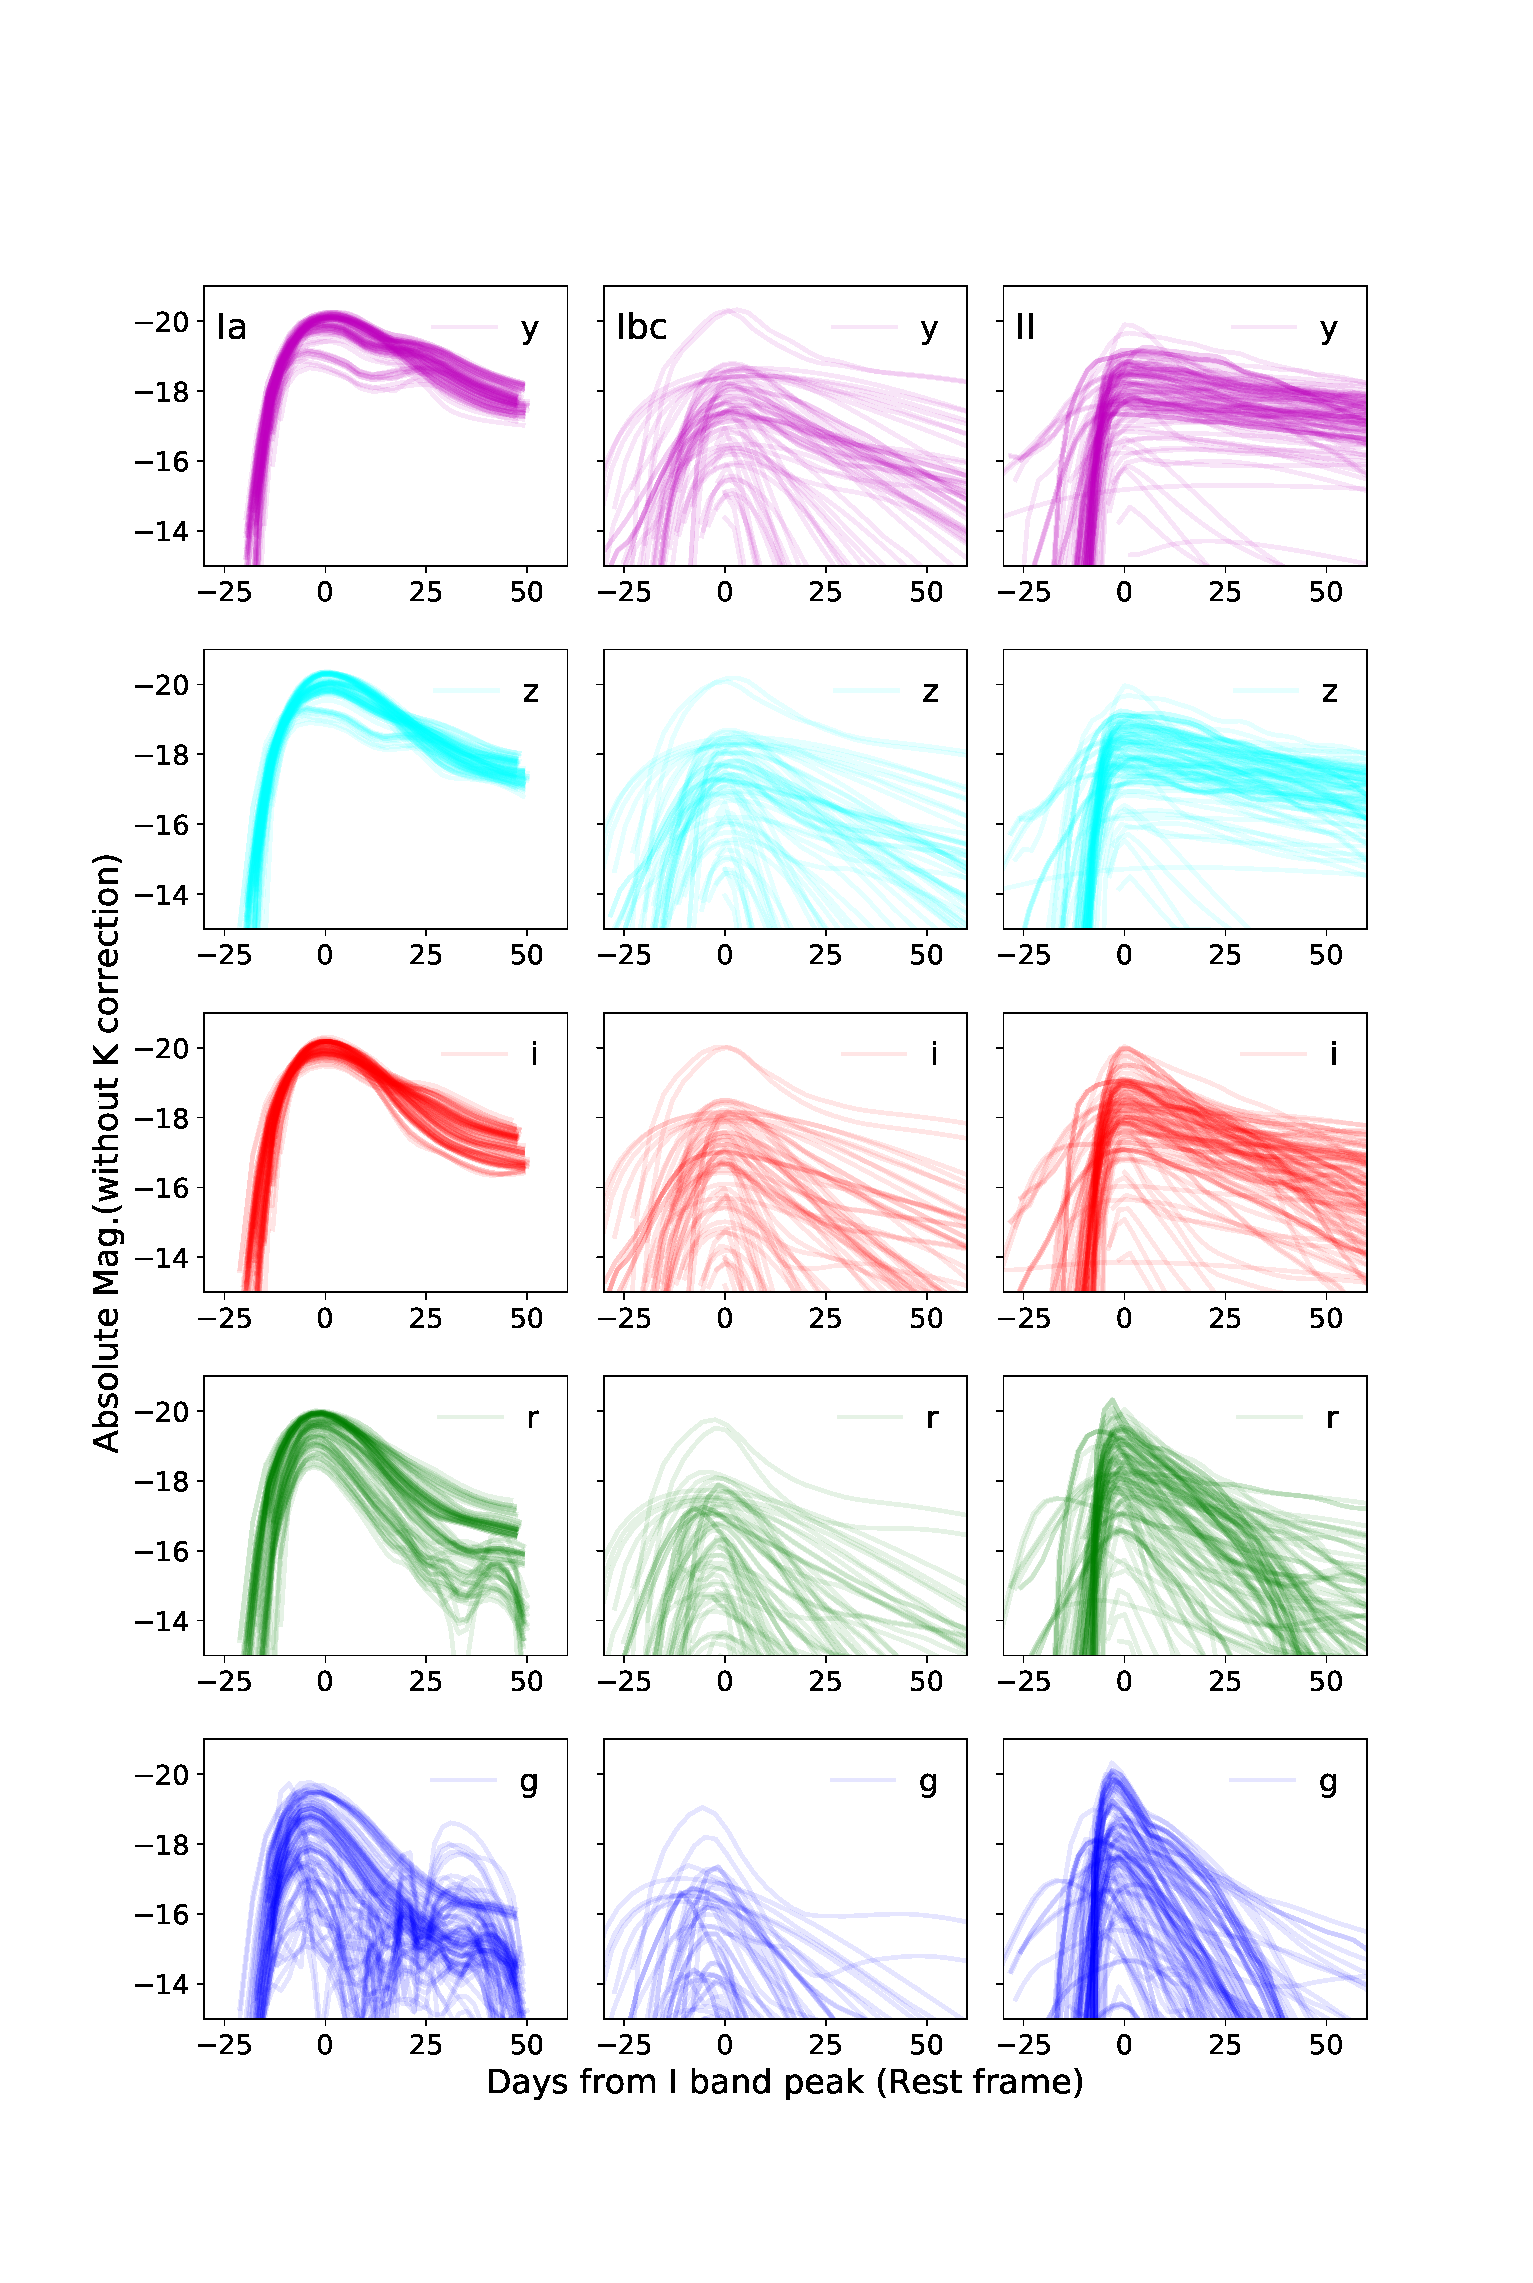
\includegraphics[width=\columnwidth]{figures/SimLCsamples.eps}
  \end{center}
  \caption{%
  Overlay plots of simulated light curves with z between 0.1 and 1.2.
  Each panel shows the case of Ia, Ibc, II from the left, and g, r, i, z, Y band from the bottom.
  No noise component is added to these light curves.
  }%
  \label{fig:simLCsamples}
\end{figure}
%
%
\subsection{Preprocessing (normazliation absolute mag)}
% われわれはシミュレーションデータを利用した実験の中で入力xは絶対等級と最大値が1になるようにスケーリングしたfluxを組み合わせるのが良いことを発見した。
% 厳密な絶対等級の計算は複雑な計算が要求されるので、簡単のために以下の式を用いた。
% また、等級の計算は観測したfluxが負の値の場合もあるので、Luptitude(Lupton magnitude)を用いて対応した。
We found that in experiments using simulation data, it is better to be input x follow as,
\begin{equation}
    x = \left( m_1^\mathrm{abs}, \ldots, m_P^\mathrm{abs}, f_{1}^{\mathrm{scale}}, \ldots, f_{P}^{\mathrm{scale}} \right)^T,
\end{equation}
where $m_i^\mathrm{abs}$ is i-th absolute magnitude, scaled flux $f_{i}^{\mathrm{scale}}$, that is,
\begin{equation}
    f_{i}^{\mathrm{scale}} = \frac{f_i}{\max \left(f_1, \ldots, f_P \right)},    \label{eq:scaled_flux}
\end{equation}
$f_i$ is i-th raw observed flux.
Since the calculation of exact absolute magnitude requires complicated calculation, the following equation is used for simplicity.
\begin{eqnarray}
    m_i^\mathrm{abs} = m_i - \mathrm{DM}\left(z\right),
\end{eqnarray}
where $m_i$ is i-th magnitude and $\mathrm{DM}\left(z\right)$ is distance modulus of the redshift value $z$.
In addition, since the observed flux may be a negative value, the calculation of the magnitude was dealt with using Luptitude (Lupton magnitude). %simplified Lupton magnitude 
\begin{eqnarray}
    m_i = 27.5 - \frac{2.5}{\log 10} \sinh^{-1} \frac{f_i}{2}. \label{eq:mag} 
\end{eqnarray}

\section{Deep Neural Network Clasifier : Imoto/Takahashi}
On the rise of the era of Big Data, the use of machine learning technique plays a critical role on the analysis of astronomical data.  Techniques such as Random Forest, Support Vector Machine, Convolution Neural Network are being used for photometric data analysis, galaxy classifications and spectral classifications.

We are in need of classifying supernova from photometric data.  We attempt to make use of the observed data as it is without parameterization.  It is the Deep Learning that makes this attempt possible.   On this paper, we test how good deep learning can do without extracting features such as color, light curve width and the peak magnitude.  It has been proven among PLAsTiCC competition that a combination of features can perform very well (cite Boone 2019), but it needs the data augmentation, interpolation or extrapolation to extract features.

We push one step further and use the observed data as raw as possible, meaning our input is a simple array of magnitudes.  Such attempt would not be possible ten years ago, but thanks for the advancement of computing and deep learning technique, now it becomes reality.  Among many other machine learning methods, deep neural network is our choice which enables us to classify astronomical objects from the raw observed data. 

\subsection{Model Design}
In this section, we describe our design of DNN model which takes an array of observed magnitudes as an input and outputs supernova classification with probabilities.  We adopted Highway Layer \citep{srivastava15a} as a core part of our network which is also called 'layer in layer'.  Compared to the plain DNN, Highway Layer can perform better when the network is deep in terms of parameter optimization \citep{srivastava15b}.   
Just like the other DNN model, this model goes through training, validation process to optimize parameters, and we describe the steps below.  The terminology we use is common in the world of DNN, but this is a new introduction to astronomical community, we spell out each step one by one.  The architecture of our model is summarized in Figure \ref{fig:dnn_model}.
At the end, each supernova is given a probability of being a certain astrophysical class, in our case, supernova types. 

{\bf Input}: Our input is an array of magnitudes and normalized flux of a supernova $i$ :
\begin{equation}
      x_i = \left( M_{i1}, M_{i2}, \ldots M_{ij} \ldots , M_{iN}, f_{i1}, f_{i2}, \ldots, f_{iN} \right)^T
\end{equation}
We do not use time or filter explicitly but it is recorded as an order inside the array.  The philosophy here is that the training set which is composed of the simulated data in the same array length holds the information on filter and dates.  For example, $j$-th magnitude in the array is the data taken on a certain date and by a certain filter.  The combination of the date and filter is identical to the ones in the training set.  Therefore, $j$-th component implicitly contains unique information about dates and filters.  
%{\bf Memo Distance Modulus \& Normalized Flux needs to be written for preprocessing}
Based on our experiment, described in $\S X$, the combination of absolute magnitude and normalized flux performs best, and therefore, our input array has a size of $1\times2N$ per a supernova where $N$ is the number of data points.
%The DNN model receives the total of P brightnesses observed in multiple bands as an input and outputs $C$ values, where $C$ is the number of classes in classification task, and $C = 1$ in regression task.

{\bf First Fully Connected Layer:}
We would like to make use of $d$ neurons which is also known as the number of 'hidden layer', and $d$ is greater than the number of input components (2$N$).  However, the dimension $d$ is not known in advance, and this is one of the hyperparameters we optimize later in this section.  Since the dimension of input (2N) and the number of optimized neurons $d$ could be different, we are in need of adjusting the dimensions and that is the role of this First Fully Connected Layer F(x).    
\begin{equation}
    F \left(x, \left\{W,b\right\}\right) = W x + b.
\end{equation}
F(x) is given by a linear combination of matrix W(2N$\times$ d) and an array b (1$\times$ d), and the initial value is generated by gaussian distribution and b is initialized by zero.  We use a python wrapper library called {\it dm-sonnet} and its function called {\it linear} supplies the F(x) when we plug in '2N' and 'd'.  The initial value of the matrix $W$ is generated by gaussian distribution and b is initialized by zero.  Later on, W and b are optimised by an open source Machine Learning package, {\it Tensorflow}.  Unless we mention otherwise, we use libraries from {\it Tensorflow}.

{\bf Dropout Layer:}
In order to have a robust result, it is always best to train the all of the neurons as an ensemble and avoid one of the neurons drags the result.  Dropout is a process which randomly drops some of the neurons from the training and the rate of dropout can be optimized as one of the hyperparameters \citep{dropout}. 

{\bf Highway layer:}
We adopted Highway Layer \citep{srivastava15a} and the number of layers is optimized through hyperparameter search.   In theory, we can design a very deep layer and the number of layers can be more than we need.   In fact, it is not trivial to find the optimized number of layers.   
%In this study, we adopted Highway Layer \citep{highway} as the basic part of the network structure.
The depth and/or layer size of the DNN model is directly related to the complexity of the features that we input, and greatly affect the performance of the task.  
However, if a model is too deep, the learning process becomes difficult and causes performance degradation.
%There are many studies to solve the problem such as optimization, initialization, and network architecture.
Highway layer is a technique that stabilizes learning process by devising the network structure.
In \citet{kimura17a}, we have used Highway Layer and tested on 2D image, and it proved a good performance.  The details of the use of Highway Layer is described in \citet{kimura17a}.  We continue to adopt Highway Layer scheme for this analysis.
%\begin{equation}
%Highway\left(h\right) = H\left(h\right) \otimes T \left(h\right) + h \otimes C\left(h\right)
%\end{equation}
%Highway layer, shown in Fig.\ref{fig:dnn_model}, has multiple paths from the input to the output.
The output of Highway Layer is calculated from the values of the multiple paths.
The output, ${\bf Highway} \left(x\right)$, is formulated as
\begin{equation}
    {\bf Highway} \left(x\right) = T \left(x\right) \cdot H \left(x\right) + C \left(x\right) \cdot x,
\end{equation}
where $H$ is a non-linear transformation layer. $T$ is the transformation gate function layer and controls the transformation of input.  $C$ is the carry gate function layer.
%The two gate functions $T$ and $C$ control how much of the outputs which are transforming the input and carrying it, respectively.
%One gate functions, $T$, controls the transformation of input and the other gate function, $C$, controls  
Highway layer includes other layers inside.  This structure is called layer in layer.  Each function is defined as follows: 
\begin{eqnarray}
    H \left(x\right) &=& \mathrm{a} \left( F \left(x, \left\{W_H, b_H\right\}\right) \right), \\
    T \left(x\right) &=& \mathrm{a} \left( F \left(x, \left\{W_T, b_T\right\}\right) \right), \\
    C \left(x\right) &=& 1 - T \left(x\right),
\end{eqnarray}
where $a$ is an activation function, namely sigmoid.
\begin{eqnarray*}
    \mathrm{a} \left(p\right) &=& \left( \sigma\left(p_1\right),\sigma\left(p_2\right), \ldots, \sigma\left(p_d\right) \right)^T, \; p \in \mathbb{R}^d, \\
    \sigma \left(p_i\right) &=& \frac{1}{1 + e^{-p_i}},
\end{eqnarray*}
Note $d$ is the number of neurons.  $T(x)$ is expected to take values between 0 and 1.  At the end values, highway layer behaves as follows:
\begin{equation}
    {\bf Highway(x)}=\left\{
    \begin{array}{@{}ll@{}}
    %\begin{cases}
      x, & \text{if}\ T \left(x\right)=0 \\
      H(x), & \text{if} \ T \left(x\right)=1 
    %\end{cases}
    \end{array}\right.
\end{equation}
% われわれはhighway blockというものを定め、highway blockの個数を変えることでネットワークの大きさを調整した。
We define a highway block which is composed of three layers: Highway Layer, Batch Normalization Layer and Activation Layer.
%and adjusted the size of the network by changing the number of highway blocks.
% highway blockは図2のようにhighway layerを含む最大で三つの層からなる。
%The highway block is composed of a maximum of three layers including a highway layer as shown in Figure \ref{fig:dnn_model}.
% ただし、highway layer以外の層については後述するハイパーパラメータ探索により決定した。
%However, layers other than Highway layer are determined by a hyperparameter search described later.
% モデルの大きさなどについてはハイパーパラメータ探索を行い決定した。
% 探索を行ったハイパーパラメータは、Highway Blockの個数$N_{block}$、Highway Blockの隠れ層の次元数$d$、ドロップアウトの割合、Batch Normalizationの有無、活性化関数の種類である。
This block itself is laid multiple times.
%and this number of blocks $N_{bloack}$ is one of the hyperparameters and optimized later. 
%The optimal structure of the network was determined by hyperparameter search.
Along with the hidden layer dimensions $d$, the dropout ratio, batch normalization, and the types of activation function, the number of highway blocks $N_{block}$ is one of the hyperparameters and optimized through hyperparameter search.   The details are described in $\S$ \ref{hyperparametersearch}.
%The subjects of hyperparameter search are the number of highway blocks $N_{block}$, the number of hidden layer dimensions $d$ of highway blocks, the dropout ratio, the presence of batch normalization, and the type of activation function.

{\bf Batch Normalization Layer:}
We adopt Batch Normalization \citep{batch_norm} to accelerate and stabilize the optimization.  Even if it may be a large number of parameters we need to train, Batch Normalization helps converge the training, reduce errors on the slope when we apply entropy minimization, prevents the average and dispersion goes exponentially large in deep layers, and minimize the biases on outputs \citep{understanding_batch_norm}.
%BNを使うと大きな学習係数でも収束する、精度が高くなるメリットがある。それは、勾配の誤差を減らせること、深い層になるほど平均と分散が指数的に大きくなるのを防げること、出力の偏りを解消することなどによる(\cite{understanding_batch_norm})。
Batch Normalization works well in many cases. However, if both Batch normalization and Dropout are in the model, the performance may degrade (\cite{dropout_and_batch_norm}).   
%ハイパーパラメータ$bn$=1ならBatch normalizationを使って、$bn$=0なら使わない。 実装はdm-sonnetのBatchNormV2クラスを利用した。

{\bf Activation Layer:}
Each neuron is activated through a non-linear transformation.  Non-linearity is an important component for DNN which gives us a wide variety of expression.   Note the majority of the layers, including Fully Connected Layers, are a linear transformation and even if we have a number of layers, it is equivalent of one single linear transformation.   Thus, it is essential to have a non-linear transformation so that each neuron can have a freedom to take any values necessary.
For the first iteration, we do not know what kind of transformation is the best, the transformation itself is taken as one of the hyperparameters.  The functions, 'tf.nn', in {\it Tensorflow} is being used.
%非線形な変換を行う。非線形な変換はDNNにおいてモデルの表現力を支える重要な要素である。Fully Connected layerをはじめとする多くのlayerは線形な変換になっている。線形なlayerのみの場合はいくらモデルを深くしようとも単一のlayerと等価なので、十分な表現力を得られない。そのため各ニューロンが様々な値を表現するために非線形な変換は必要である。
%変換の種類は何が良いかわからないので、恒等変換も含めてその変換の種類をハイパーパラメータとして後述の方法で最適化した。
%実装はtf.nnの中にあるそれぞれの関数を利用した。

{\bf Second Fully Connected Layer:}
%D次元からC次元に隠れ層の次元数を変換する。
After Highway Layer Block is stacked for 3-5 times, we are in need of converting the number of neurons to the number of supernovae times the number of supernova classes.   This is an opposite operation of the first fully connected layers.

{\bf Softmax layer}
softmax layer normalize the value $h$ with following formula,
\begin{equation}
    \hat{y}_j = \frac{\exp \left( h_j \right)}{\sum_{k=1}^C \exp \left( h_k \right)}.
\end{equation}
The normalized value $\hat{y}$ satisfies $\hat{y}_j \geq 0$ and $\sum_j^C \hat{y}_j =1$.
We can interpret $\hat{y}_j$ as the probability that the input $x$ belongs to  class $c=j$.
  
\subsection{Hyper Parameter Search}\label{hyperparametersearch}
% fig.\ref{fig:dnn_model}の赤色の背景の値をDNNの精度が最も高くなるように決定する。ハイパーパラメータの値とDNNの精度の関係を陽に求めることは非常に難しく計算コストも高いので、それらの間の関係はブラックボックスとしてハイパーパラメータの最適化を行う。
% 今回、われわれは最初にグリッドサーチを行い、その後、TPEアルゴリズムによる探索を行った。グリッドサーチは探索点を任意に指定できることと複数の点の評価を同時に行えるので時間的な効率が良いことから採用した。また、TPEアルゴリズムは探索履歴に基づいて次の探索点を決定するので、履歴にグリッドサーチの結果を含めることでグリッドサーチでは見つけられなかったより良い点を探索できる。
% グリッドサーチの探索グリッドは予備実験で良かった点とその周辺の点を設定した。各グリッド点の評価は並列で行った。
% ハイパーパラメータの探索にはグリッドサーチとTPE(Tree-structured Parzen Estimator)アルゴリズムを組み合わせる方法で行った。
We performed hyperparameter search by combining grid search and TPE (Tree-structured Parzen Estimator) algorithm.
% グリッドサーチは高次元空間の探索はあまり適していないが、並列に複数の点を探索できるメリットがある。
Grid search is not suitable for high-dimensional space search, but has the advantage of searching for multiple points in parallel.
% 加えて、アルゴリズムが単純なので、予備実験の結果などの知見を探索点の設定に反映させやすいメリットがある。
In addition, since the algorithm is simple, there is a merit that it is easy to reflect knowledge such as the results of preliminary experiments in the setting of search points.
% 一方で、TPEアルゴリズムは高次元空間の探索に適しているが、現在までの探索結果に基づいて次の探索点を決定するので探索が逐次的になるデメリットがある。
On the other hand, the TPE algorithm is suitable for searching a high-dimensional space, but has a demerit that the search is sequential because the next search point is determined based on the search results up to now.
% そこで今回は予備実験でよかったハイパーパラメータの周辺をグリッドサーチで探索を行い、続いてその結果に基づいてTPEアルゴリズムでの探索を行った。
Therefore, this time, we searched around the hyperparameters that were good in the preliminary experiment by grid search, and then searched by TPE algorithm based on the result.
% 組み合わせることで、予備実験で得た知識を利用でき、探索にかかる時間を短縮できるメリットがある。
By combining them, there are merits that the knowledge obtained in the preliminary experiment can be used and the time required for the search can be shortened.

%% DNNのハイパーパラメータはoptunaを用いて最適化を行った。
% ハイパーパラメータの最適化は、学習用データセットを訓練データとバリデーションデータに分割して、バリデーションデータでの精度が最も高くなるように最適化した。
% 最適化によって得られたハイパーパラメータを用いてモデルの最適化を行い、そのモデルの性能の評価を行った。
%% note: 参考文献にはOputunaのソースコード https://github.com/pfnet/optunaではなく、元論文の方を指定した
% We optimized the hyperparameters of the DNN model using the library, optuna(\cite{optuna}).
In optimizing the hyperparameters, we evaluated the hyperparameters with validation accuracy.
We divided the data set into training data and validation data.
We used training data for optimizing DNN and used validation data for measuring the accuracy.
We trained the DNN model using the hyper parameters obtained by optimization, and evaluated the performance of the DNN model.

%\section{Results (TBD Experiment/Execution)}
\begin{figure}[ht]
  \begin{center}
     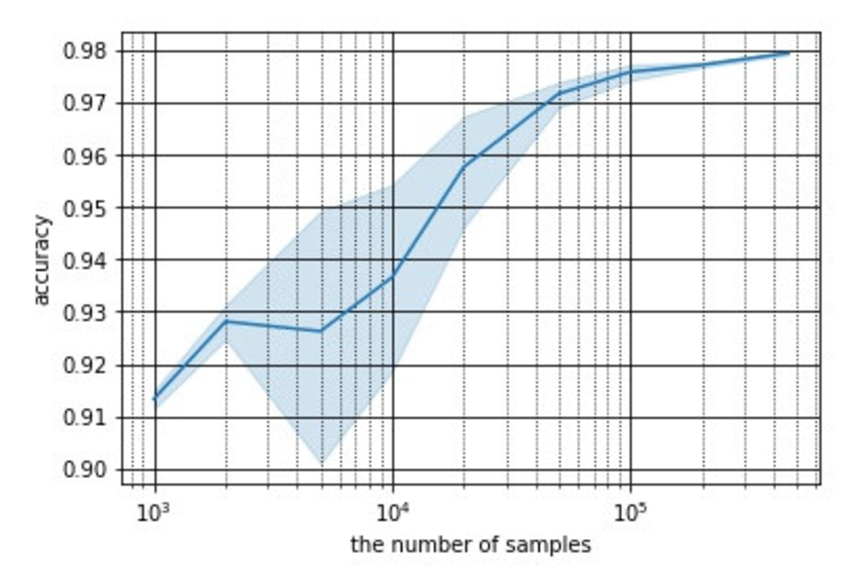
\includegraphics[width=\columnwidth]{figures/size_accuracy.eps}
  \end{center}
  \caption{%
  the relation between the number of samples of training dataset and the accuracy measured with test dataset. The solid line shows the mean accuracy of five classifiers. The shade area shows the standard deviation of the classifiers. The classifiers are trained with 5 fold cross validation using the training dataset. (The validation data is used to stop the training.)
  }%
  \label{fig:size_convergence_test}
\end{figure}
\begin{figure}[ht]
  \begin{center}
     \includegraphics[width=\columnwidth]{figures/hp_iterations_accuracy.eps}
  \end{center}
  \caption{%
  binary classification, flag=0
  }%
  \label{fig:size_convergence_test}
\end{figure}
%
%\subsubsection{}


\begin{figure}[ht]
  \begin{center}
     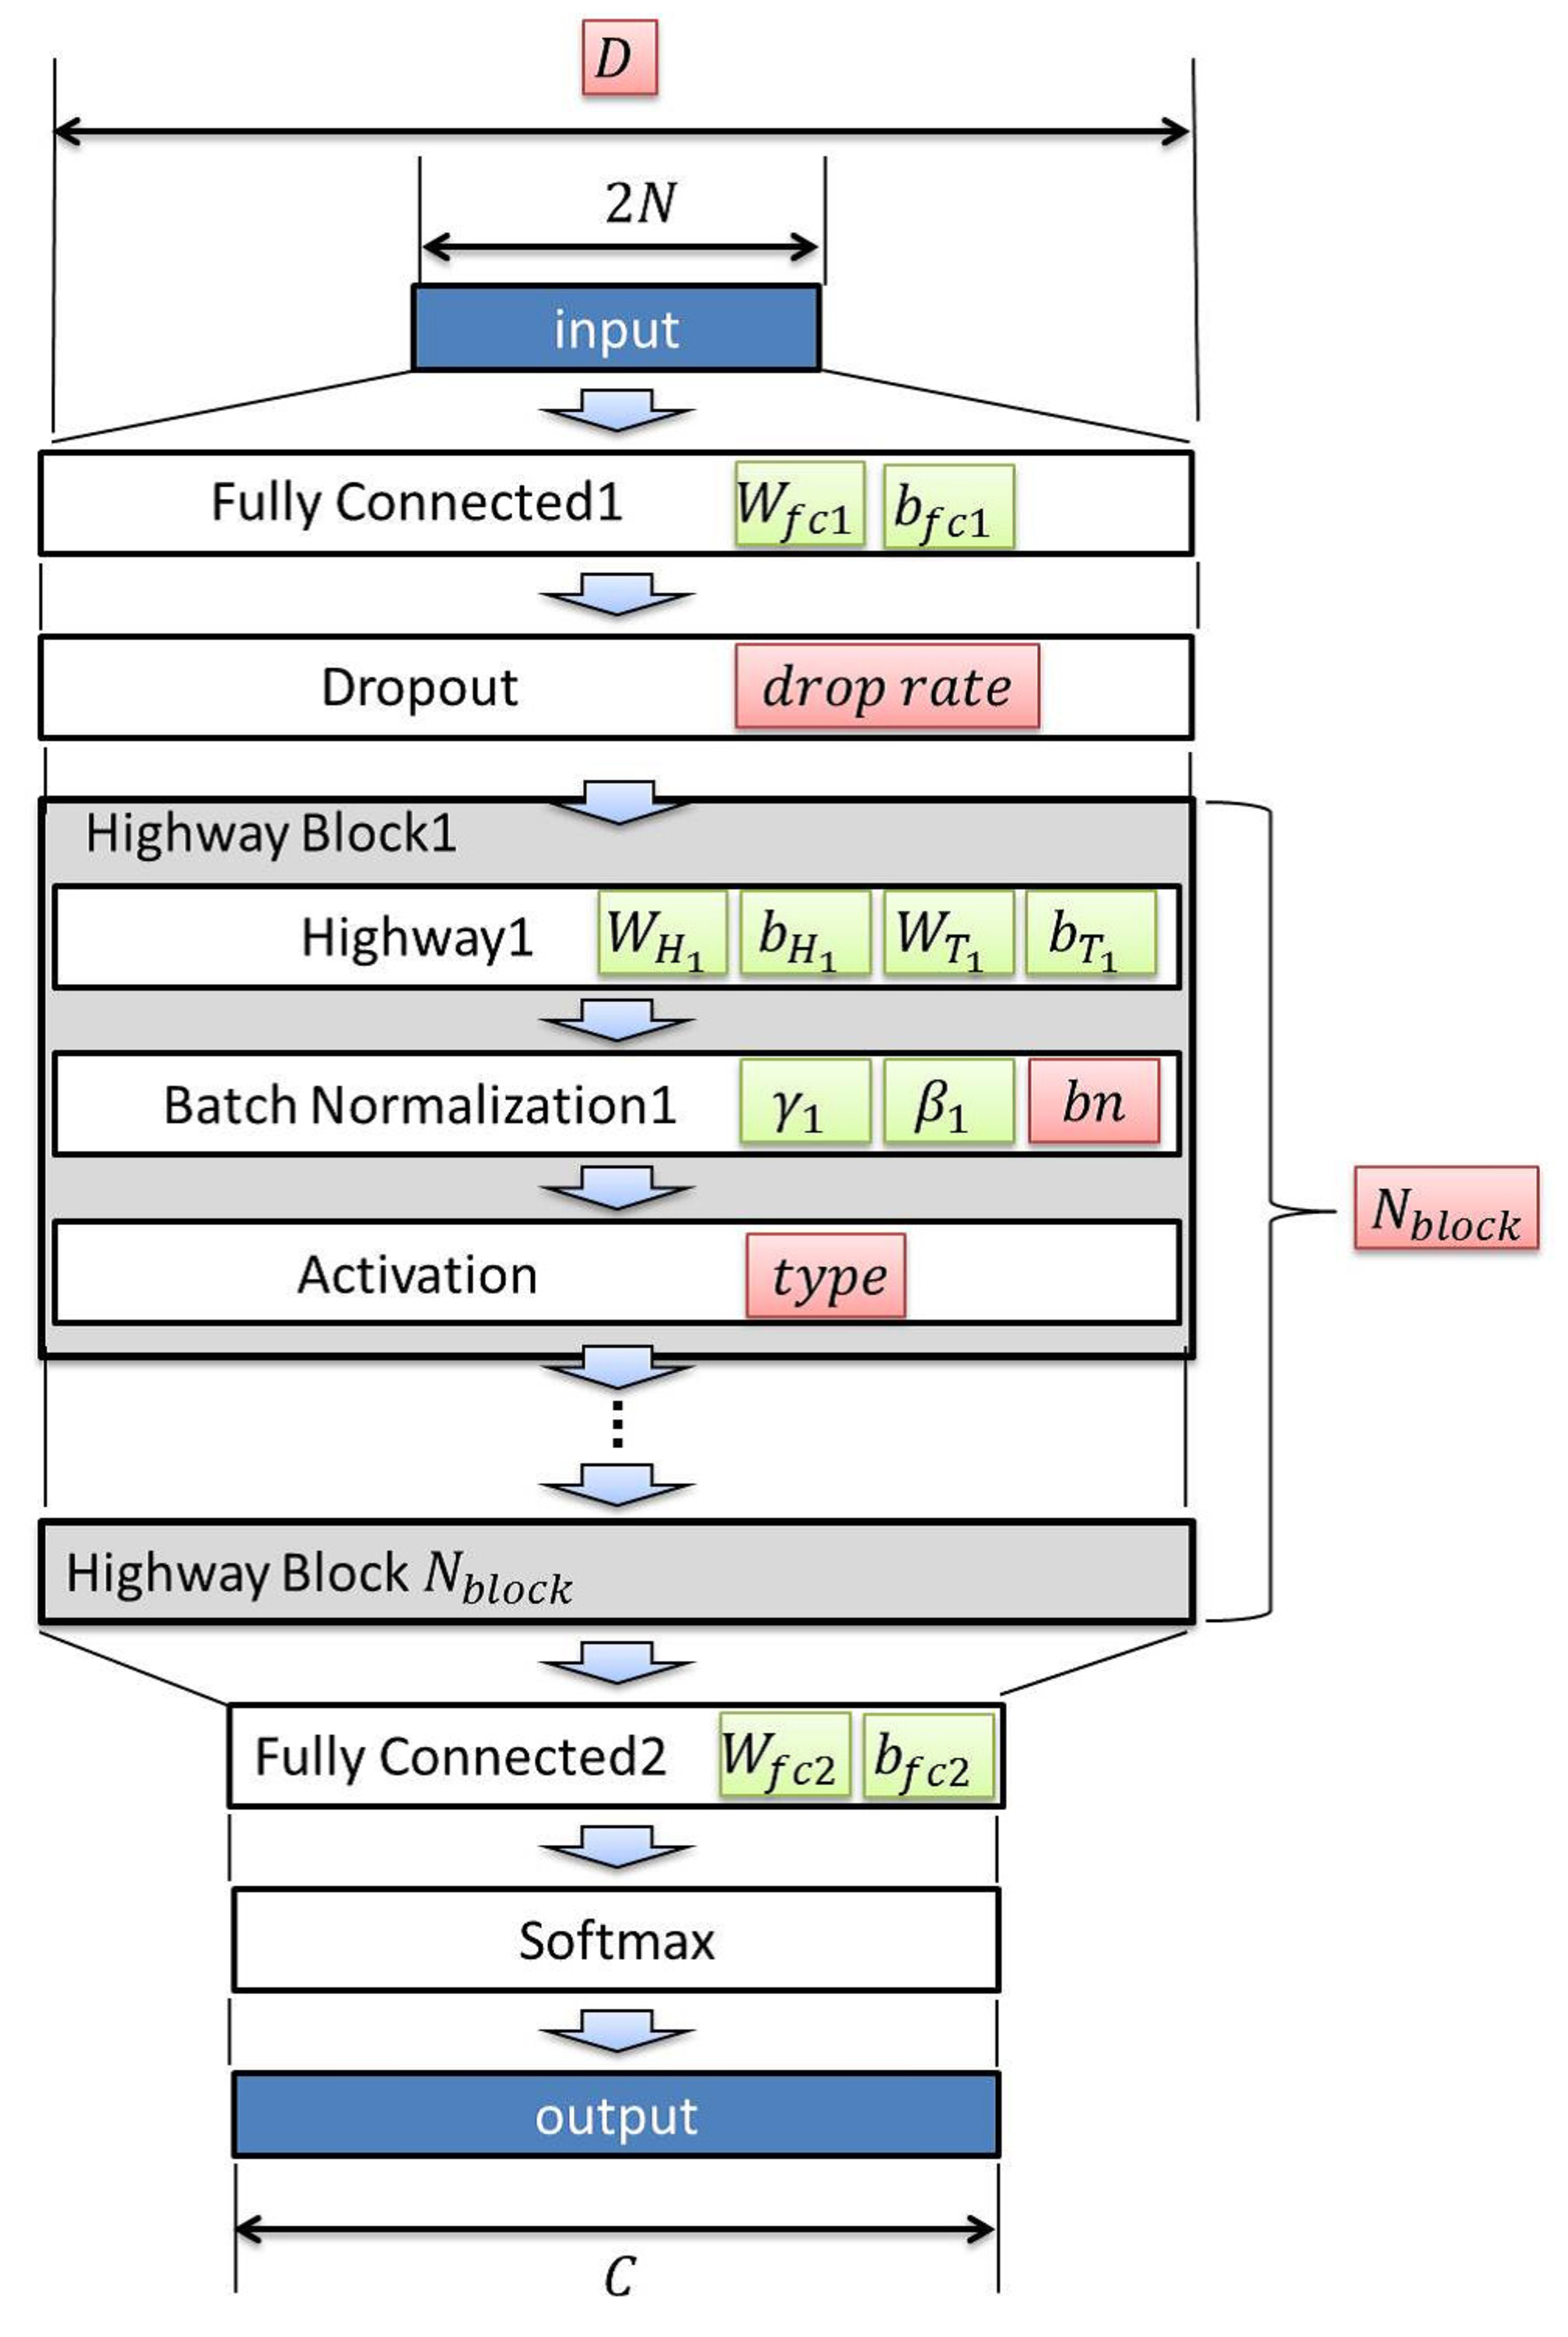
\includegraphics[width=\columnwidth]{figures/model_all.eps}
  \end{center}
  \caption{\label{dnnmodel}
  The architecture of the deep neural network classifier. 
  The green boxes are parameters which are optimized by gradient descent method during training. The red boxes are hyper-parameters which are optimized by the hyper-parameter search. 
  Batch normalization layer has four variables ($\mu, \sigma^2, \gamma, \beta$). $\mu$ and $\sigma^2$ are to learn the statistics (mean and variance) of the value through the layer respectively.  $\gamma$ and $\beta$ are scale parameter and shift parameter to adjust the output. $\mu$ and $\sigma^2$ are are not updated by gradient descent method and are updated by moving average. We omit them from the figure for simplicity.
  }%
  \label{fig:dnn_model}
\end{figure}

\begin{table*}[t]
  \tbl{Optimized hyper-parameters for the classification}{
      \begin{tabular}{lcccllllllllll}
\hline
%      & $M$        & $m$        & $f$        & the number of blocks T & hidden size D & drop rate & bn & type    \\ \hline
      & \multicolumn{3}{l}{Input}            & \multicolumn{5}{l}{Two-Class}      &  \multicolumn{5}{l}{Three-Class}   \\ \hline
      & $M$        & $m$        & $f$        & T & D   & drop rate & bn & type    & T & D   & drop rate & bn & type    \\ \hline      
flag0 & \checkmark &            & \checkmark & 5 & 178 & 9.47e-3   & 1  & sigmoid & 4 & 429 & 1.20e-3   & 0  & linear  \\
      & \checkmark &            &            & 3 & 247 & 9.68e-4   & 1  & sigmoid & 4 & 516 & 2.54e-3   & 0  & tanh    \\
      &            & \checkmark & \checkmark & 4 & 531 & 6.43e-3   & 0  & linear  & 4 & 608 & 1.72e-2   & 0  & linear  \\
      &            & \checkmark &            & 4 & 411 & 9.00e-2   & 1  & sigmoid & 4 & 838 & 1.36e-3   & 0  & tanh    \\ \hline
flag1 & \checkmark &            & \checkmark & 5 & 734 & 8.75e-4   & 0  & tanh    & 4 & 915 & 1.03e-2   & 0  & linear  \\
      & \checkmark &            &            & 2 & 389 & 7.17e-2   & 1  & sigmoid & 5 & 698 & 2.79e-2   & 0  & linear  \\
      &            & \checkmark & \checkmark & 2 & 647 & 7.92e-4   & 0  & tanh    & 4 & 540 & 1.45e-3   & 0  & linear  \\
      &            & \checkmark &            & 2 & 342 & 1.42e-2   & 1  & sigmoid & 2 & 520 & 9.99e-4   & 1  & sigmoid \\ \hline
flag2 & \checkmark &            & \checkmark & 2 & 368 & 1.79e-3   & 1  & sigmoid & 4 & 698 & 9.08e-4   & 0  & linear  \\
      & \checkmark &            &            & 4 & 920 & 1.44e-3   & 0  & sigmoid & 4 & 614 & 7.03e-3   & 0  & linear  \\
      &            & \checkmark & \checkmark & 5 & 572 & 4.27e-3   & 1  & sigmoid & 4 & 896 & 8.58e-3   & 0  & linear  \\
      &            & \checkmark &            & 4 & 640 & 1.12e-1   & 1  & sigmoid & 5 & 300 & 5.00e-1   & 1  & sigmoid \\ \hline
flag3 & \checkmark &            & \checkmark & 5 & 893 & 1.42e-3   & 1  & sigmoid & 4 & 522 & 5.02e-4   & 0  & tanh    \\
      & \checkmark &            &            & 4 & 880 & 1.98e-2   & 1  & sigmoid & 5 & 841 & 4.96e-2   & 1  & sigmoid \\
      &            & \checkmark & \checkmark & 3 & 300 & 5.00e-3   & 1  & linear  & 3 & 462 & 9.28e-4   & 1  & sigmoid \\
      &            & \checkmark &            & 3 & 930 & 9.77e-2   & 1  & sigmoid & 3 & 300 & 5.00e-3   & 1  & sigmoid \\ \hline
flag4 & \checkmark &            & \checkmark & 5 & 379 & 4.21e-3   & 1  & sigmoid & 3 & 484 & 2.13e-3   & 0  & linear  \\
      & \checkmark &            &            & 2 & 631 & 1.77e-2   & 0  & sigmoid & 4 & 243 & 3.21e-3   & 1  & sigmoid \\
      &            & \checkmark & \checkmark & 5 & 140 & 4.04e-3   & 1  & sigmoid & 5 & 389 & 1.23e-4   & 0  & tanh    \\
      &            & \checkmark &            & 4 & 567 & 5.77e-2   & 0  & sigmoid & 3 & 354 & 2.14e-1   & 1  & sigmoid \\ \hline
\end{tabular}
  }\label{tb:searched_hp_class}
\end{table*}

%
% このセクションでは超新星のタイプ分類とredshiftの推定に利用した手法について説明する。
% 続いて、モデルの学習方法とモデルのハイパーパラメータの決定方法についても説明する。
%In this section, we describe the method used for supernova type classification and regression of the value of redshift.
%Next, we will explain how to learn the model and how to determine the hyperparameters of the model.

%DNN is one of machine learning methods inspired by the biological brain system.
%DNN combines a large number of elements that mimic neurons, and each element has only a simple function, but it can obtain complex functions as a whole.
% DNNは明示的に特徴を与えることなく、与えられた入力から目的のタスクを解くために必要な特徴を自動的に獲得する
%DNN model can obtain the features needed to solve the target task from the given input without explicitly giving the features.
%Our goal is to classify the type of the celestial body or to estimate the redshift value from the observed light curve.
% われわれはlight curveのタイプ分類にdeep neural network(DNN)を利用した。
% このDNNは、複数のバンドで観測された合計M個の明るさを入力として$K$個の値を出力する。ここで、$K$はクラス数である。
%We used DNN model for them.
%The DNN model receives the total of P brightnesses observed in multiple bands as an input and outputs $C$ values, where $C$ is the number of classes in classification task, and $C = 1$ in regression task.
% 本研究ではfig \ref{fig:dnn_model} に示す構造のモデルを利用した。
%We used the structural model shown in Fig.\ref{fig:dnn_model}.

% 本研究ではネットワーク構造の基本的な部分にHighway Layerを採用した
% dnnモデルの深さや層の大きさはその獲得できる特徴の複雑さに直結して、タスクに対しての性能にも大きく影響する
% 一方で、深すぎるモデルは学習が困難になり、かえって性能の低下を引き起こす
% その問題の解決のためにoptimizer、初期化、ネットワーク構造の工夫など、数多くの研究が存在する
% Highway layerはネットワークの構造を工夫することで学習を安定化させる手法である。
%In this study, we adopted Highway Layer \citep{highway} as the basic part of the network structure.
%The depth and/or layer size of the DNN model are directly related to the complexity of the features that can be obtained, and greatly affect the %performance for the task.
%However, a too deep model is difficult to learn and rather causes performance degradation.
%There are many studies to solve the problem, such as optimization, initialization, and network architecture.
%Highway layer is a technique that stabilizes learning by devising the network structure.

% highway layerは図2に示す通り、入力から出力までの経路が複数存在している。
% highway layerの出力はその複数の経路の値から作られる。
% 出力は以下の式であらわされる。

%Highway layer, shown in Fig.\ref{fig:dnn_model}, has multiple paths from the input to the output.
%The output of Highway Layer is calculated from the values of the multiple paths.
%The output, ${\bf Highway} \left(x\right)$, is formulated as
%\begin{equation}
%    {\bf Highway} \left(x\right) = T \left(x\right) \cdot H \left(x\right) + C \left(x\right) \cdot x,
%\end{equation}
%where $H$ is a non-linear transformation layer, $T$ is the transformation-gate function layer, and $C$ is the carry-gate function layer.
%The two gate functions $T$ and $C$ control how much of the outputs which are transforming the input and carrying it, respectively.
%Highway layer includes other layers inside.
%This structure is called layer in layer.

%We defined the functions as 
%\begin{eqnarray}
%    H \left(x\right) &=& \mathrm{a} \left( F \left(x, \left\{W_H, b_H\right\}\right) \right), \\
%    T \left(x\right) &=& \mathrm{a} \left( F \left(x, \left\{W_T, b_T\right\}\right) \right), \\
%    C \left(x\right) &=& 1 - T \left(x\right),
%\end{eqnarray}
%where $a$ is an activation function, that is,
%\begin{eqnarray*}
%    \mathrm{a} \left(z\right) &=& \left( \sigma\left(z_1\right),\sigma\left(z_2\right), \ldots, %\sigma\left(z_d\right) \right)^T, \; z \in \mathbb{R}^d, \\
%    \sigma \left(z_i\right) &=& \frac{1}{1 + e^{-z_i}},
%\end{eqnarray*}
%$d$ is the size of the dimension of the input and the output of Highway Layer, and
%$F$ is a fully connected layer parameterized by $W \in \mathbb{R}^{d \times d}$ and $b \in \mathbb{R}^d$, is formulated as
%\begin{equation}
%    F \left(x, \left\{W,b\right\}\right) = W x + b.
%\end{equation}
%Fully connected layer is a popular and basic layer of DNN.
%This formulation of Highway layer is same as (\cite{highway}).

% 二つの値の混ぜ合わせによって、highway layerの出力が作られる。
% ゲートT=1の場合は通常のfully conected layerと等しい。
% 逆にC=1の場合は恒等変換でlayerがないのと等しく、ネットワークの実質的な深さが減少する。この場合、浅いネットワークと同じで学習しやすくなる。
% ゲートの値は[0, 1]の連続値なので、実際には中間的な振る舞いになる。この時の振る舞いも中間的なものになる。
% highway layerの二つのgate function, T and Cよって出力が調整される。
% 恒等変換の出力は層がない状態と等しいのでモデルの実質的な深さを減らす効果がある。
% このゲートの働きによってHighway layerの出力は非線形は変換と恒等変換の中間的なものになる。
% layerの出力が恒等変換であればネットワークの深さが実質的に減少することになる。



\subsubsection{Binary and Multi-type}
% DNNでのクラス分類は、DNNの各出力を各クラスに対応させることで、クラス数$K$によらずに同じ方法で学習できる。
% 多クラス分類の場合は、我々の実験ではクラス数が$K=3$なので、出力数も3となる。
% 同様にbinaryクラス分類では出力数は2となる。
We can train the DNN classifier in the same way regardless of the number of classes.
In the case of multi-type classification, the number of classes is $K = 3$ in our experiment, so the number of outputs of the DNN classifier is also three.
Similarly, in binary classification, the number of the outputs is two.

% モデルの学習はクロスエントロピー誤差$CE \left( t, y \right) = -\sum_{k=1}^K t_k \log y_k$を最小化するようにした。
% $t$は$k$次元のone hotベクトルで正解のクラス$k$に対応する次元のみが1、残りは全て0のベクトルである。
% $y$はDNNの出力ベクトルである。
% モデルのパラメータの更新は勾配法でadam optimizerを利用して行った。
We trained the model as minimizing the cross-entropy error 
\begin{equation}
\mathrm{CE} \left(y, \hat{y} \right) = -\sum_{k = 1}^K y_k \log \hat{y}_k,
\end{equation}
where $y$ is a ground truth vector which is one-hot encoding of $K$ dimension, and $\hat{y}$ is the DNN output vector.
We used Adam optimizer, which is a kind of stochastic gradient method, to update model parameters.

% 学習時のオーバーフィッティングを防ぐためにdata augmentationを行った。
We performed data augmentation to prevent overfitting in training time.
% data augmentationによって見かけのデータ数を増やすことで、DNNが訓練データを暗記してしまうのを防ぐ効果がある。
By increasing the number of apparent data by data augmentation, there is an effect to prevent DNN from memorizing training data.
% 学習データに2種類のdata augmentationを適用した。
We applied two kinds of data augmentation to the learning data.
% 一つはfluxにガウス分布からサンプリングしたノイズを加えた。
One is that the noise sampled from Gaussian distribution is added to flux
% もう一つはmixup (\cite{mixup})を行った。
The other is mixup (\cite{mixup}).

% ノイズの追加は、以下のように、eq.\ref{eq:scaled_flux}, eq.\ref{eq:abs_mag}において$\hat{f}_i$を$\hat{f}_i + \epsilon_i$で置き換えた。ここで、$\epsion_i \sim \mathcal{N} \left(0, e_i\right)$、$\mathcal{N}\left(\bullet, \bullet\right)$は標準正規分布、$e_i$は$\hat{f}_i$に対応するflux eroorである。
To add noise to flux, as follows, we replaced $f_i$ with $f_i + \epsilon_i$ in eq.\ref{eq:scaled_flux} and eq.\ref{eq:mag},
where $\epsilon_i$ is a random noise drawn from the Gaussian distribution with zero mean and $e_i^2$ variance, and $e_i$ is the flux error corresponding to $f_i$.
Mixup generates new virtual training examples as follows:
\begin{eqnarray*}
    \tilde{x} &=& \lambda x_s + \left( 1-\lambda \right) x_t, \\
    \tilde{y} &=& \lambda y_s + \left( 1-\lambda \right) y_t,
\end{eqnarray*}
where $\left(x_s, y_s\right)$ and $\left(x_t, y_t\right)$ are samples drawn at random from the training dataset, $x$ is input vector, $y$ is one-hot label vector, and a mixing ratio $\lambda \in \left[0, 1\right]$ is drawn from a random distribution which is low density around 0 and 1 and higher density around 0.5. 
The generated samples are suitable for DNN to learn the classification boundaries.

% 前述のとおり、モデルのハイパーパラメータは探索を行い決定した。
As described above, the hyperparameters of the model were determined by searching.
% グリッドサーチの設定は表1の通りで、TPEアルゴリズムでの探索の設定は表2のとおりである。
%Table\ref{tb:hp_grid} shows the grid search settings, and Table\ref{tb:hp_search} shows the search settings for the TPE algorithm.
Table\ref{tb:hp} shows the grid search settings and the search settings for the TPE algorithm.
% われわれはハイパーパラメータ探索によってクラス分類に最適なDNNの大きさを決定した。
% モデルの良さを測る尺度には学習に用いなかったバリデーションデータの精度とした。
% われわれはハイパーパラメータ探索の第一段階として表?の値のデカルト積で作られる各要素についてグリッド探索を行った。
% 続いて表?の範囲についてTPEアルゴリズムで探索を行った。
% We determined the optimal DNN model size for classification by hyperparameter search.
% The scale for measuring the goodness of the model was the accuracy of the validation data, which was not used for training.
% As the first step of hyperparameter search, we performed a grid search for each element created by Cartesian product of the values in Table \ref{tb:hp_grid}.
% Subsequently, we searched in the range in Table \ref{tb:hp_search} using the TPE algorithm.

% DNNの学習は5-fold cross validationで行い、その5つの学習器による予測結果の平均で評価した。
% DNNの予測ベクトルのうちで最も値が高い要素に対応するクラスをDNNが予測したクラスとする。
% DNNの予測したクラスと正解ラベルの一致率で精度を評価する。
% The performance evaluation of the models was performed by 5-fold cross validation.
% Let the class corresponding to the element with the highest value among the prediction vector be the class predicted by DNN.
% The accuracy is evaluated by the matching rate of DNN predicted class and the ground truth.

\begin{table}[ht]
  \tbl{Settings of hyper parameter search in type classification}{
      \begin{tabular}{lcc}
        \hline
        hyper parameter     & value (grid)  & range (TPE)\\ \hline 
        D                   & \{100, 300\}  & 50, \ldots, 1000   \\
        T                   & \{1, 3, 5\}   & 1, \ldots, 5       \\
        bn                  & \{true\}      & \{true, false\}    \\
        dropout rate        & [5e-3, 0.035] & [5e-4, 0.25]       \\
        activation function & \multicolumn{2}{c}{\{identity, relu, sigmoid, tanh\}} \\
        \hline
      \end{tabular}
  }\label{tb:hp}
\end{table}

\begin{comment}
% ハイパーパラメータ探索の初期で探索する各ハイパーパラメータの候補
\begin{table}[ht]
  \tbl{The settings of hyper parameter search}{
      \begin{tabular}{lc} 
        \hline
        hyper parameter & value \\ \hline 
        hidden size & \{100, 300\} \\
        the number of highway layers & \{1, 3, 5\} \\
        use of batch normalization & \{true\} \\
        dropout rate & [5e-3, 0.035] \\
        activation function & \{identity, relu, sigmoid, tanh\} \\
        \hline
      \end{tabular}
  }\label{tb:hp_grid}
\end{table}
% ハイパーパラメータの一覧
\begin{table}[ht]
  \tbl{The settings of hyper parameter search}{
      \begin{tabular}{lc} 
        \hline
        hyper parameter & range or candidates \\ \hline 
        hidden size & 50, \ldots, 1000 \\
        the number of highway layers & 1, \ldots, 5 \\
        use of batch normalization & \{true, false\} \\
        dropout rate & [5e-4, 0.25] \\
        activation function & \{identity, relu, sigmoid, tanh\} \\
        \hline
      \end{tabular}
  }\label{tb:hp_search}
\end{table}
% 
\end{comment}
%
%
\begin{figure}[ht]
  \begin{center}
     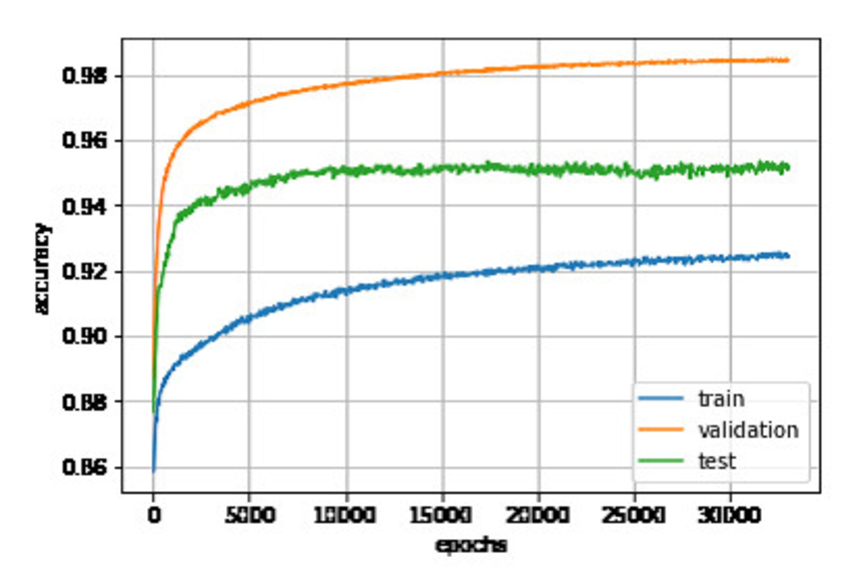
\includegraphics[width=\columnwidth]{figures/abs_mag-sflux-accuracy.eps}
  \end{center}
  \caption{%
  accuracy
  }%
  \label{fig:abs_mag-sflux-accuracy}
\end{figure}
%
%

\subsubsection{Regression of Redshift Value}

% 観測した明るさからその天体のredshiftを推定した
% DNNの出力がスカラーになって最後のsoftmat layerがないことを除けば、図2と同じ構造のモデルを利用した。
% モデルの最適化は正解のredshiftの値と出力値の二乗誤差を小さくするようにした。
% モデルのハイパーパラメータについてはクラス分類の時と同様に行った。
% 表?の値のデカルト積で作られる要素をグリッドサーチ、続いて表?の範囲の中をTPEアルゴリズムで探索を行った。
% ハイパーパラメータの最適化は$R^2$決定係数を最大にするようにした。
We estimated the redshift value $z$ of the object from the observed brightness。
We cannot use absolute magnitude to estimate the redshift value because redshift value is required to calculate absolute magnitude.
Therefore, we used magnitude instead of absolute magnitude as the input of the DNN.

We used a model with the same structure as in fig.\ref{fig:dnn_model} except that the DNN output was a scalar and there was no final softmax layer for redshift estimation.
The objective function to optimize is the squared error between the ground truth $z$ and the output value $\hat{y}$.
We measured the accuracy of the model with the coefficient of determination $R^2$, that is,
\begin{eqnarray*}
    R^2 = 1 - \frac{\sum_n \left| z_n - \hat{y}_n \right|^2}{\sum_n \left| z_n - \bar{z} \right|^2}, 
\end{eqnarray*}
where $z_n$ is the redshift value of n-th sample, $\hat{y}_n$ is the output of n-th sample, and $\bar{z}$ is the mean redshift of the dataset.
% $\mathrm{SE} \left(z, y\right) = \frac{1}{2} \left| z - y \right|^2 $
We performed hyperparameter search in the model as in the case of classification.
%The element created by the Cartesian product of the values in Table \ref{tb:hp_grid_redshift} was searched by grid search, and then the range in Table \ref{tb:hp_search_redshift} was searched by the TPE algorithm.
The search values, ranges and candidates are surmalized in Table \ref{tb:hp_redshift}.
% 学習時にfluxにノイズを加えるdata augmentationを行った。一方で、クラス分類の場合とは異なりmixupは行っていない。
We performed data augmentation that adds noise to the flux in training time.
On the other hand, unlike the case of classification, no mixup is performed.

\begin{table}[ht]
  \tbl{Settings of hyper parameter search in redshift estimation}{
     \begin{tabular}{lcc} 
        \hline
        hyper parameter     & value (grid)    & range (TPE)\\ \hline 
        D                   & \{750, 1500\}   & 100, \ldots, 3000   \\
        T                   & \{3, 5, 7\}     & 3, \ldots, 7        \\
        bn                  & \{true, false\} & \{true, false\}     \\
        dropout rate        & 1e-3            & [5e-4, 0.25]        \\
        activation function & \multicolumn{2}{c}{\{identity, relu, sigmoid, tanh\}} \\
        \hline
      \end{tabular}
  }\label{tb:hp_redshift}
\end{table}

\begin{comment}
% ハイパーパラメータ探索の初期で探索する各ハイパーパラメータの候補
\begin{table}[ht]
  \tbl{The settings of hyper parameter search}{
     \begin{tabular}{lc} 
        \hline
        hyper parameter & value \\ \hline 
        hidden size & \{750, 1500\} \\
        the number of highway layers & \{3, 5, 7\} \\
        use of batch normalization & \{true, false\} \\
        dropout rate & 1e-3 \\
        activation function & \{identity, relu, sigmoid, tanh\} \\
        \hline
      \end{tabular}
  }\label{tb:hp_grid_redshift}
\end{table}
% redshiftの推定のハイパーパラメータの一覧
\begin{table}[ht]
  \tbl{The settings of hyper parameter search}{
      \begin{tabular}{lc} 
        \hline
        hyper parameter & range or candidates \\ \hline 
        hidden size & 100, \ldots, 3000 \\
        the number of highway layers & 3, \ldots, 7 \\
        use of batch normalization & \{true, false\} \\
        dropout rate & [5e-4, 0.25] \\
        activation function & \{identity, relu, sigmoid, tanh\} \\
        \hline
      \end{tabular}
  }\label{tb:hp_search_redshift}
\end{table}
%
\end{comment}

\section{Validation with PLAsTiCC data} %Takahashi
%
We verify the performance of the classifier described in the previous section using the PLAsTiCC dataset.
PLAsTiCC data is mainly divided into two components, Wide-Fast-Deep (WFD) and Deep-Drilling-Fields (DDF), based on survey styles with different cadences.
WFD data is not suitable for classification by our proposed method, because it consists of a group of light curves simulated assuming a wide area survey of almost half of the whole sky, and have various observation schedules.
In contrast, DDF data is suitable for the verification of our method because it has photometric data that simulates the observation of specific areas with the same cadence as the HSC survey.
Therefore, we validated the classifier using DDF data which have the fixed observation schedule for each object.
About 2300 events extracted from PLAsTiCC DDF data were used for the test set.
These are three types of supernovae, Ia, Ibc, and II, which are simulated to occur in the COSMOS field, the target region of HSC survey.
For these events, we extracted only the light curves for about one year during which supernovae occur from the original three-year data and input them into the classifier.
%
We prepared several classifiers with different inputs for comparison.
Specifically, there are two types of inputs, magnitude or absolute magnitude, and a total of four types of classifiers including cases where scaled flux is added to the input. 
We tried two cases of classification tasks: two-class classification to classify Ia or non Ia and three-class classification to classify Ia, Ibc or II.
We evaluated the results by Area Under the Curve (AUC) of Receiver Operating Characteristic (ROC) curve and Precision-recall curve in two-class classification, and calculated accuracy from confusion matrix in three-class classification.
%
\subsection{Simulated data}
%\begin{itemize}
%\item Flow of simulated data classification
%\item Distribution of predictions in redshift (figure?)
%\end{itemize}
%
Prior to validation of PLAsTiCC data, we evaluated classification performance for simulated lightcurves by performing cross-validation on approximately 370,000 events simulated using PLAsTiCC template.
The simulated light curve has a class ratio of Ia : Ibc : II = 0.60 : 0.06 : 0.34, and the positions of these peaks are randomly shifted between 450 days.
Table\ \ref{tab:p_validation} shows the AUC of ROC curve and Precision recall curve in two-class classification, and accuracy in three-class classification.
The classifier given absolute magnitudes and normalized flux performed best in both two-class and three-class in the simulated data classification.
The accuracy in the three-class classification is 97.8\%.
From these results, we confirmed that the classifier can classify simlated data with high accuracy.
%There is almost no difference in performance between the two input type models of magnitude and absolute magnitude.
%It may be necessary to summarize the ratio of each class
%
%
%
%PLAsTiCC, validation(v1.2.1)
%
\begin{table}[ht]
\tbl{Classification performance of each input for the PLAsTiCC validation dataset.}{
\begin{tabular}{cccccc}
\hline
\multicolumn{3}{c}{Input}   & \multicolumn{2}{c}{AUC} & Accuracy \\
\hline
%\begin{tabular}{c}absolute\\magnitude\end{tabular} & magnitude & \begin{tabular}{c}normalized\\flux\end{tabular} &  ROC &  PreRec &\\
$M$ & $m$ & $f$ &  ROC &  Pre.-Rec. &\\
\hline
\checkmark &            & \checkmark &    1.000 &       1.000 &     0.985\\
\checkmark &            &            &    0.999 &       1.000 &     0.975\\
           & \checkmark & \checkmark &    0.999 &       0.999 &     0.975\\
           & \checkmark &            &    0.998 &       0.999 &     0.956\\
\hline
\end{tabular}
}\label{tab:p_validation}
\end{table}
%
%
\subsection{PLAsTiCC data}
%\begin{itemize}
%\item Validation using a part of samples with answers
%\item ROC curve and Precision-Recall curve in binary classification(figure)
%\item Confusion matrix in 3 class classification(figure)
%\item Comparison with the 1st model in PLAsTiCC (If possible)
%\item 
%\end{itemize}
Whereas we extracted and classified a part of the simulated data for learning in the previous subsection, here we verify the classification performance for PLAsTiCC data.
We used simullate data for learning, and compared the classification result for PLAsTiCC data with true label.
Tables \ref{tab:p_test} show the AUC in two-class classification and Accuracy in three-class classification in PLAsTiCC data, respectively.
As with the case of the simulated data, the classifier with absolute magnitudes and normalized flux provides the best classification results for PLAsTiCC data.
The AUC for the ROC curve and Precision recal curve are 0.996 and 0.995 respectively.
%, and these curves in this model are shown in figure\ \ref{fig:plasticc_2class_ROC} and figure\ \ref{fig:plasticc_2class_PreRec}.
Figure\ \ref{fig:plasticc_3class_CM} shows the confusion matrix in the three-class classification, and the total accuracy is calculated as 95\%.
Although the classification performance for Ibc is not high, since the number of them is small, the effect on total accuracy is relatively small.
%
%
%PLAsTiCC, test(v1.2.1)
%
\begin{table}[ht]
\tbl{Classification performance of each input for the PLAsTiCC test dataset.}{
\begin{tabular}{cccccc}
\hline
\multicolumn{3}{c}{Input}   & \multicolumn{2}{c}{AUC} & Accuracy \\
\hline
%\begin{tabular}{c}absolute\\magnitude\end{tabular} & magnitude & \begin{tabular}{c}normalized\\flux\end{tabular} &  ROC &  PreRec &\\
$M$ & $m$ & $f$ &  ROC &  Pre.-Rec. &\\
\hline
\checkmark &            & \checkmark &    0.996 &       0.995 &     0.953\\
\checkmark &            &            &    0.995 &       0.993 &     0.952\\
           & \checkmark & \checkmark &    0.995 &       0.993 &     0.948\\
           & \checkmark &            &    0.995 &       0.991 &     0.940\\
\hline
\end{tabular}
}\label{tab:p_test}
\end{table}
%
\begin{figure}[ht]
  \begin{center}
     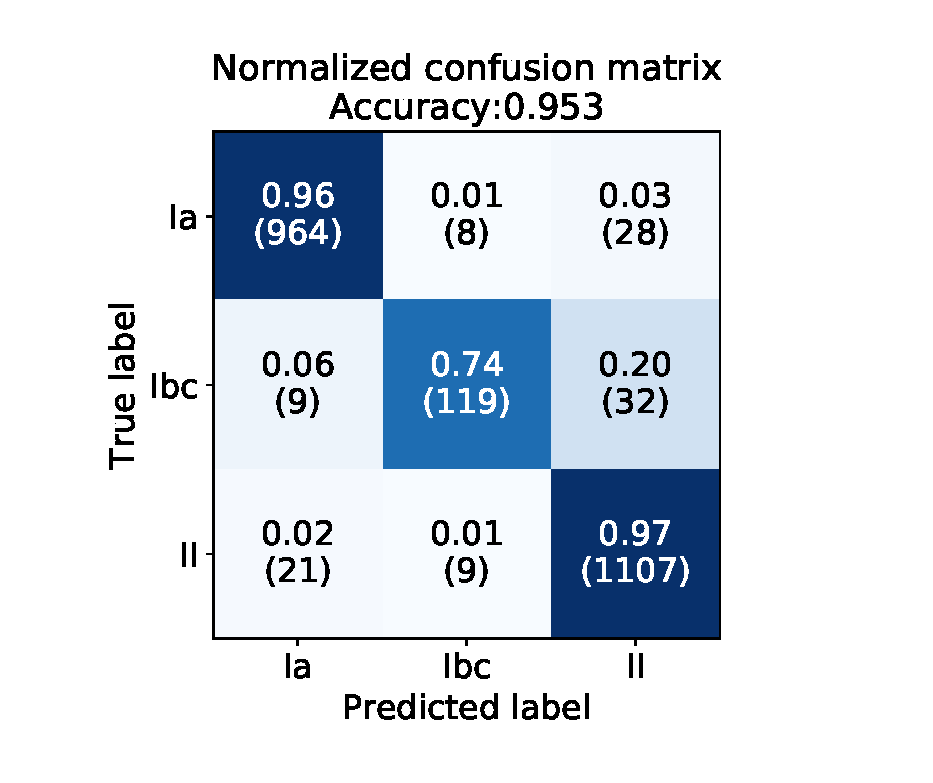
\includegraphics[width=\columnwidth]{figures/06_CM_abs-mag_scaled-flux_w-mixup_predictions_test_2.eps}
  \end{center}
  \caption{%
  Confusion matrix in three-class classification of PLAsTiCC test set.
  The number and the number in parentheses in each box represent the ratio for true label and the raw number.
  }%
  \label{fig:plasticc_3class_CM}
\end{figure}
%
%%%%%%%%%%%%%%%%%%%%%%%%%%%%%%%%%%%%%%%%%%%%
\section{Application to HSC survey}
%
We applied the developed classifier to the light curve data of supernovae discovered in the HSC transient survey.
The classifier was trained using approximately 520,000 simulated light curve data created in the same way as PLAsTiCC data classification.
Their class ratio is Ia: Ibc: II = 0.59 : 0.07 : 0.34, and the shift range of the peaks is the same as that of PLAsTiCC data, 450 days.
We used 1824 supernovas detected in the survey as a test set.
They have 42 epochs of photometric data in four bands of g, r, i, z excluding Y band.
Because part of the y-band photometric data has residuals due to improper background subtraction influenced by scattered light,
%need reference
We exclude the Y band data, considering the impact on classification performance.
The number of epochs and the schedule for each filer are summarized in Table\ \ref{tab:HSCsurvey_schedule}.
%
\begin{table}[ht]
\tbl{Number of epochs and the schedule for each filer.}{
\begin{tabular}{lcc}
\hline
Filter & epochs & Elapsed day \\
\hline
g & 8 & -57, -19, 4, 11, 33, 60, 67, 95 \\
r & 9 & -54, -27, 2, 12, 33, 44, 63, 70, 92 \\
i & 13 & -57, -53, -27, -19, 2, 9, 12, 35, 42, 61, 68, 95, 96 \\
z & 12 & -59, -53, -29, -19, 0, 9, 31, 42, 60, 67, 92, 98 \\
%Y  & 10 & -59, -26, -17, 4, 13, 37, 45, 59, 68, 89 \\
\hline
\end{tabular}
}\label{tab:HSCsurvey_schedule}
\end{table}
%

%Explanation of Flags (difference in input epochs)
Because observations were performed in two areas with different observation frequencies, "Deep" area and "Ultra Deep" area, the number of photometric data of supernova in these areas is different.
There are also events in which part of the light curve data is missing.
To correspond these supernovae, we prepared five input patterns of light curve data and classifiers for each pattern.
The number of supernovae for each pattern are summarized in Table\ \ref{tab:class_flag}.
The combination of these classifiers enables the classification of 1812 supernovae corresponding to 99.3\% of all target supernovae.
The remaining 12 supernovae are excluded in this classification because they have many missing data.
We applied both two-class and three-class classification tasks to HSC data, as with PLAsTiCC data.
%
\begin{table}[ht]
\tbl{Number of supernovae for each pattern.}{
\begin{tabular}{lrrrr}
\hline
Flag & Epoch & Number & Cumulate & Cumulate ratio \\
\hline
0     & 52      & 709        & 709         & 0.389 \\
1     & 32      & 646        & 1355       & 0.743 \\
2     & 23      & 271        & 1626       & 0.891 \\
3     & 12      & 122        & 1748       & 0.958 \\
4     & 6        & 64        & 1812       & 0.993 \\
\hline
\end{tabular}
}\label{tab:class_flag}
\end{table}
%
%%%%%%%%%%%%%%%%%%%%%%%%%%%%%%%%%%%%%%%%%%%%%%%%%
\subsection{Binary classification}
%
In binary classification, we prepared four versions of classifiers with different inputs as in PLAsTiCC data, and compared their performance.
%The performance for each input of binary classification are summarized in Table\ \ref{tab:h2_validation},\ref{tab:h2_test_gold} and \ref{tab:h2_test_all}.
The performance for each input of binary classification are summarized in Table\ \ref{tab:h2_AUC}.
For the validation dataset, the higher the number of input dimensions, the better the results, and any classifier can classify them with very high AUCs.
The AUCs for all classified events are 0.993 and 0.995 for the ROC curve and precision-recall curve, respectively.
%Figure\ \ref{fig:h2_validation} show ROC curves and precision-recall curves in the best performing classifier for the validation set.
For the test set, the classification performance is verified assuming that the classes of 1540 supernovae labeled by the SALT2 light curve fitter \citep{guy2007}, one of the conventional classification methods, is correct.
In addition, we extracted 441 "gold samples" that have redshift estimated from the spectrum and have photometric information before and after peak, and also verified their classification results.
Figures\ \ref{fig:h2_test_all} and \ref{fig:h2_test_gold} show the AUCs of the best classifier for all labeled supernovae and gold samples respectively.
The confusion matrices for each case are shown in Figure\ \ref{fig:h2_test_CM}.
%need reference
The best performing classifier shows the same classification results as the conventional method with an accuracy of 82\% for all labeled supernovae and 91\% for the gold samples.
The final classification result of the HSC supernovae is the combination of outputs from the classifier using the absolute magnitude for those with redshift information, and from that using the magnitude for those without redshift information.
The numbers of supernovae classified as Ia by the classifier are 613, 437, and 186 out of 1540 when the threshold value of Ia probability are 0.5, 0.7, and 0.9, respectively.
%
% completeness and purity
%
%
%
%2class AUC
%Ver. 1.2.0 
\begin{table*}[h]
\tbl{AUC of each input in the HSC binary classification.}{
\begin{tabular}{c|ccc|p{2em}p{2em}p{2em}p{2em}p{2em}p{2em}|p{2em}p{2em}p{2em}p{2em}p{2em}p{2em}}
\hline
Dataset & \multicolumn{3}{c}{Input} & \multicolumn{6}{|c|}{ROC} & \multicolumn{6}{c}{Pre.-Rec.} \\
\hline
 & $M$ & $m$ & $f$ & Flag0 & Flag1 & Flag2 & Flag3 & Flag4 & All & Flag0 & Flag1 & Flag2 & Flag3 & Flag4 & All \\
\hline
Validation &\checkmark &            & \checkmark &       1.000&       0.990 &       0.987 &       0.976 &       0.887 &        0.993 &          1.000 &          0.993 &          0.991 &          0.983 &          0.917 &           0.995 \\
& \checkmark &            &            &       0.999&       0.980 &       0.975 &       0.959 &       0.845 &        0.987 &          0.999 &          0.986 &          0.982 &          0.972 &          0.886 &           0.991 \\
&           & \checkmark & \checkmark &       0.999&       0.983 &       0.979 &       0.963 &       0.817 &        0.988 &          0.999 &          0.988 &          0.985 &          0.973 &          0.863 &           0.992 \\
&           & \checkmark &            &       0.996&       0.971 &       0.966 &       0.938 &       0.790 &        0.980 &          0.997 &          0.980 &          0.976 &          0.955 &          0.841 &           0.985 \\
\hline
Test& \checkmark &            & \checkmark &       0.972 &       0.973 &       0.946 &       0.889 &       1.000 &        0.966 &          0.918 &          0.956 &          0.860 &          0.838 &          1.000 &           0.919 \\
(Gold sample)& \checkmark &            &            &       0.979 &       0.974 &       0.977 &       0.900 &       0.944 &        0.972 &          0.938 &          0.942 &          0.960 &          0.870 &          0.908 &           0.936 \\
&           & \checkmark & \checkmark &       0.934 &       0.928 &       0.886 &       0.711 &       0.889 &        0.918 &          0.798 &          0.852 &          0.791 &          0.605 &          0.579 &           0.795 \\
&           & \checkmark &            &       0.926 &       0.887 &       0.868 &       0.822 &       0.611 &        0.894 &          0.757 &          0.775 &          0.775 &          0.693 &          0.374 &           0.751 \\
\hline
Test& \checkmark &            & \checkmark &       0.919 &       0.906 &       0.896 &       0.862 &       0.849 &        0.903 &          0.769 &          0.785 &          0.758 &          0.708 &          0.598 &           0.759 \\
(All sample)& \checkmark &            &            &       0.921 &       0.910 &       0.884 &       0.863 &       0.864 &        0.902 &          0.786 &          0.772 &          0.701 &          0.757 &          0.658 &           0.742 \\
&           & \checkmark & \checkmark &       0.877 &       0.868 &       0.852 &       0.703 &       0.724 &        0.853 &          0.644 &          0.689 &          0.678 &          0.441 &          0.302 &           0.632 \\
&           & \checkmark &            &       0.868 &       0.827 &       0.830 &       0.683 &       0.675 &        0.831 &          0.620 &          0.624 &          0.623 &          0.408 &          0.293 &           0.601 \\
\hline
\end{tabular}
}\label{tab:h2_AUC}
\end{table*}
\begin{comment}
%
%Validation
%
\begin{figure*}[h]
    \begin{tabular}{cc}
        \begin{minipage}{0.5\hsize}
            \begin{center}
                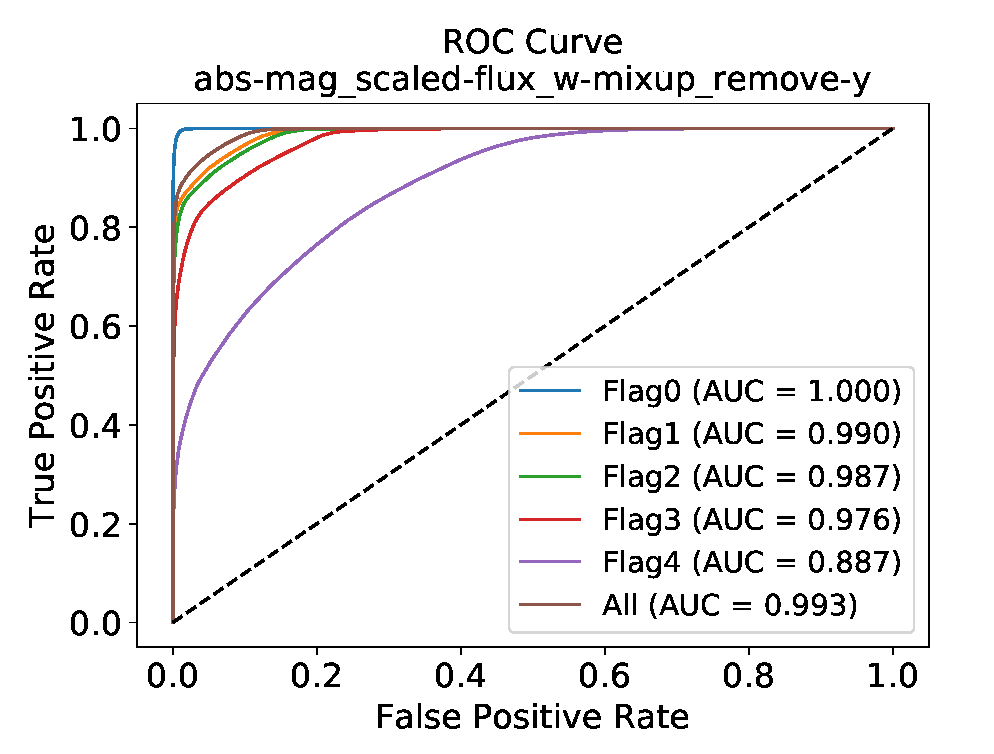
\includegraphics[width=\columnwidth]{figures/08_abs-mag_scaled-flux_w-mixup_remove-y_predictions_validation_ROC.eps}
            \end{center}
        \end{minipage}
        \begin{minipage}{0.5\hsize}
            \begin{center}
                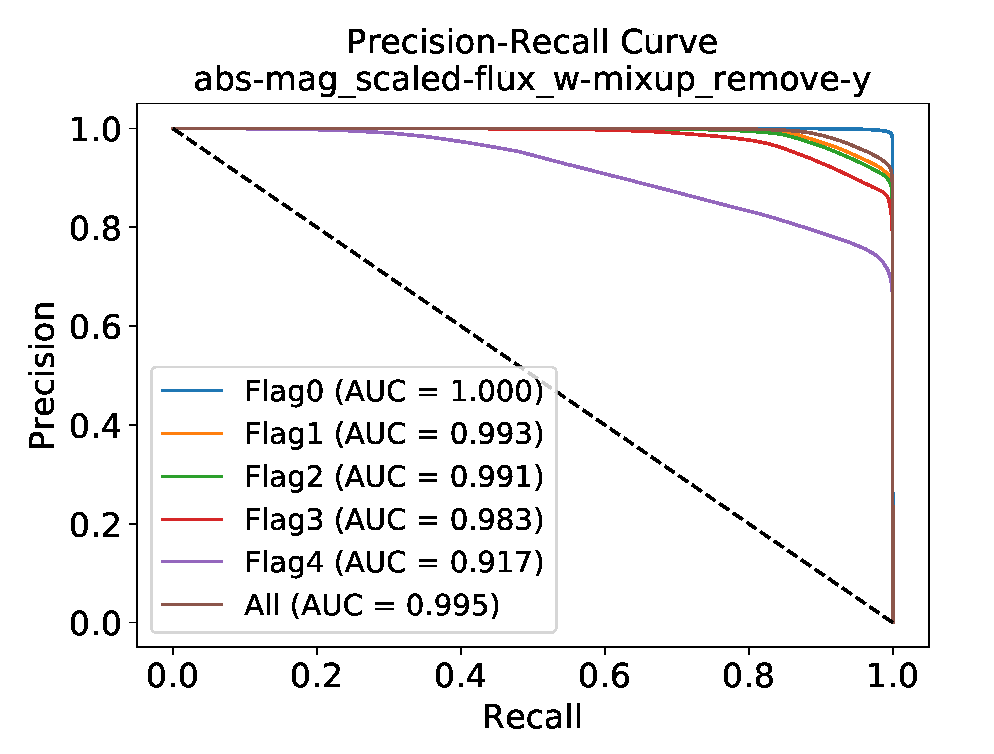
\includegraphics[width=\columnwidth]{figures/08_abs-mag_scaled-flux_w-mixup_remove-y_predictions_validation_PreRec.eps}
            \end{center}
        \end{minipage}
    \end{tabular}
    \caption{%
  ROC curves and precision Recall curves in two-class classification of validation dataset.
}%
    \label{fig:h2_validation}
\end{figure*}
\end{comment}
%
% all samples
%
%
\begin{figure*}[h]
    \begin{tabular}{cc}
        \begin{minipage}{0.5\hsize}
            \begin{center}
                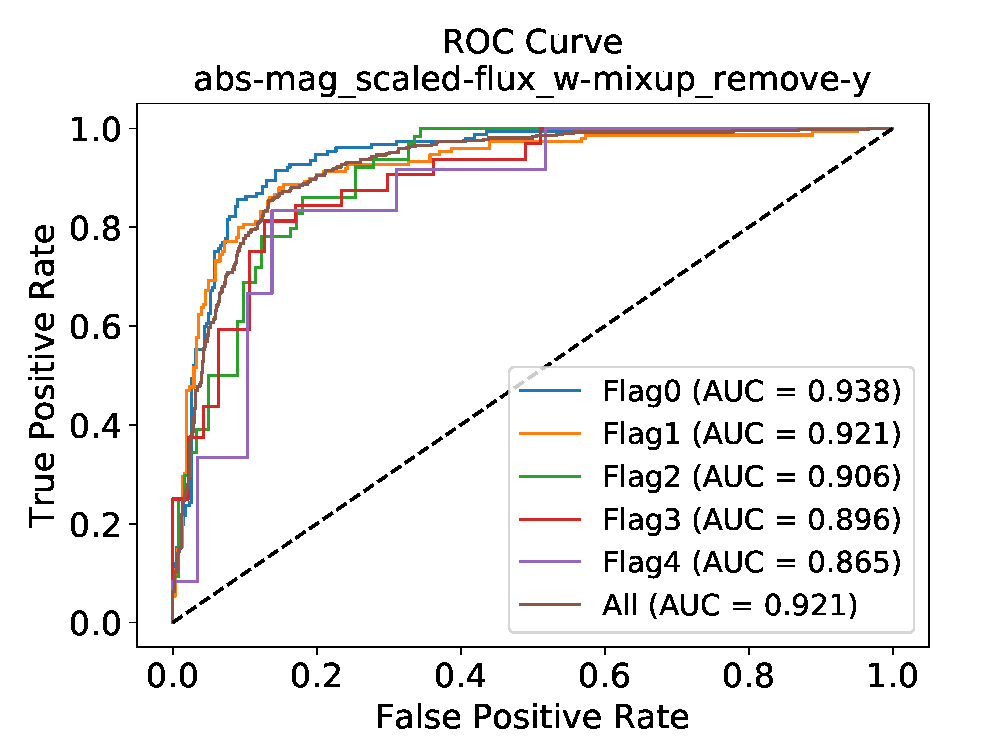
\includegraphics[width=\columnwidth]{figures/10_abs-mag_scaled-flux_w-mixup_remove-y_predictions_test_ROC_all.eps}
            \end{center}
        \end{minipage}
        \begin{minipage}{0.5\hsize}
            \begin{center}
                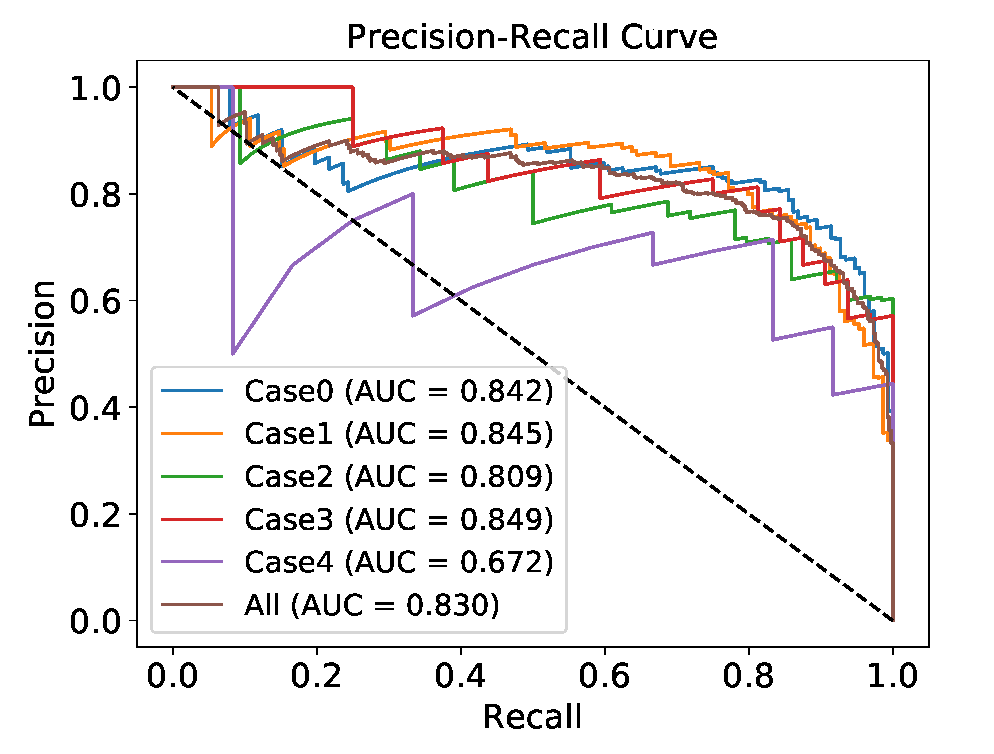
\includegraphics[width=\columnwidth]{figures/10_abs-mag_scaled-flux_w-mixup_remove-y_predictions_test_PreRec_all.eps}
            \end{center}
        \end{minipage}
    \end{tabular}
    \caption{%
    ROC curves and precision Recall curves in two-class classification of test dataset(All samples).
    }
    \label{fig:h2_test_all}
\end{figure*}
%
%
%spec-z \& w/o edge samples
%
\begin{figure*}[ht]
    \begin{tabular}{cc}
        \begin{minipage}{0.5\hsize}
            \begin{center}
                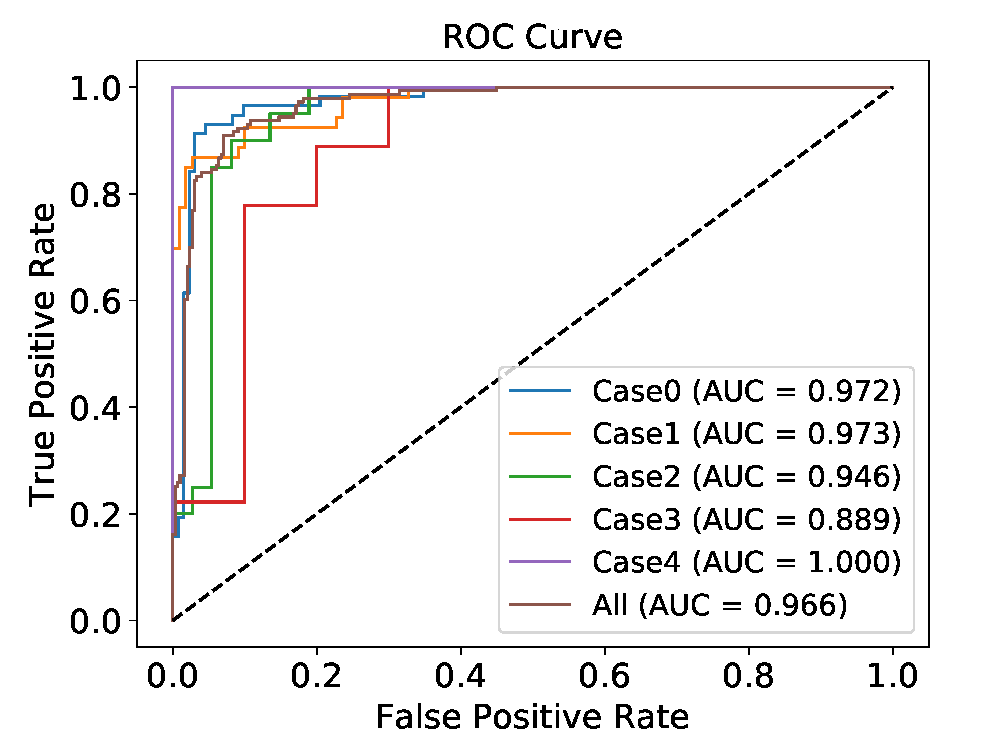
\includegraphics[width=\columnwidth]{figures/10_abs-mag_scaled-flux_w-mixup_remove-y_predictions_test_ROC_noedge_spec.eps}
            \end{center}
        \end{minipage}
        \begin{minipage}{0.5\hsize}
            \begin{center}
                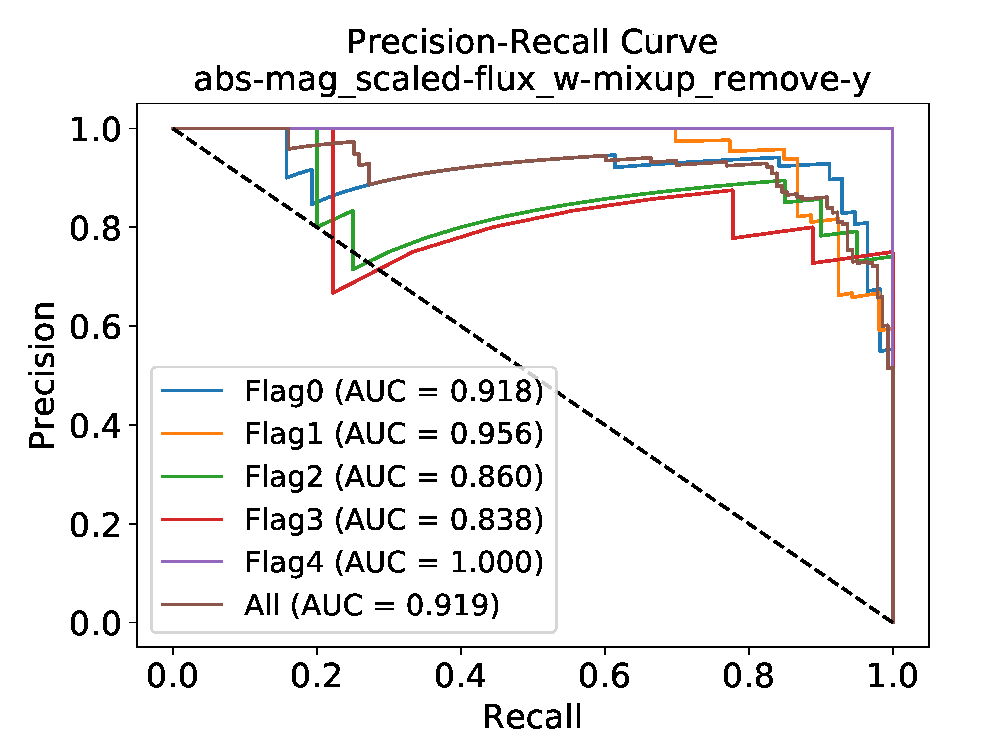
\includegraphics[width=\columnwidth]{figures/10_abs-mag_scaled-flux_w-mixup_remove-y_predictions_test_PreRec_noedge_spec.eps}
            \end{center}
        \end{minipage}
    \end{tabular}
    \caption{%
  ROC curves and precision Recall curves in two-class classification of test dataset(Gold samples).
}%
    \label{fig:h2_test_gold}
\end{figure*}
%
%
\begin{comment}
%2class Test Accuracy
%Ver. 1.2.0
%
%% spec-z & w/o edge samples
%
\begin{table*}[ht]
\tbl{Accuracy of each input in the HSC binary classification.}{
\begin{tabular}{c|ccc|p{2em}p{2em}p{2em}p{2em}p{2em}p{2em}}
\hline
Dataset & \multicolumn{3}{|c}{Input} & \multicolumn{6}{|c}{Accuracy} \\
\hline
 & $M$ & $m$ & $f$  &  Flag\_0 &  Flag\_1 &  Flag\_2 &  Flag\_3 & Flag\_4 &  All \\
\hline
Test& \checkmark &            & \checkmark &        0.947 &        0.902 &        0.877 &        0.789 &        0.923 &         0.914 \\
(Gold sample)& \checkmark &            &            &        0.931 &        0.902 &        0.912 &        0.789 &        0.769 &         0.907 \\
&           & \checkmark & \checkmark &        0.878 &        0.847 &        0.825 &        0.632 &        0.538 &         0.839 \\
&           & \checkmark &            &        0.868 &        0.816 &        0.789 &        0.842 &        0.462 &         0.825 \\
\hline
Test& \checkmark &            & \checkmark &        0.859 &        0.816 &        0.757 &        0.778 &        0.745 &         0.818 \\
(All sample)& \checkmark &            &            &        0.843 &        0.778 &        0.734 &        0.697 &        0.618 &         0.784 \\
&           & \checkmark & \checkmark &        0.798 &        0.782 &        0.767 &        0.636 &        0.508 &         0.765 \\
&           & \checkmark &            &        0.790 &        0.744 &        0.737 &        0.645 &        0.393 &         0.740 \\
\hline
\end{tabular}
}\label{tab:h2_test_CM}
\end{table*}
\end{comment}
%
%
%2class Test CM
%Ver. 1.2.0
%
%% spec-z & w/o edge samples
%
\begin{figure*}[ht]
    \begin{tabular}{cc}
        \begin{minipage}{0.5\hsize}
            \begin{center}
                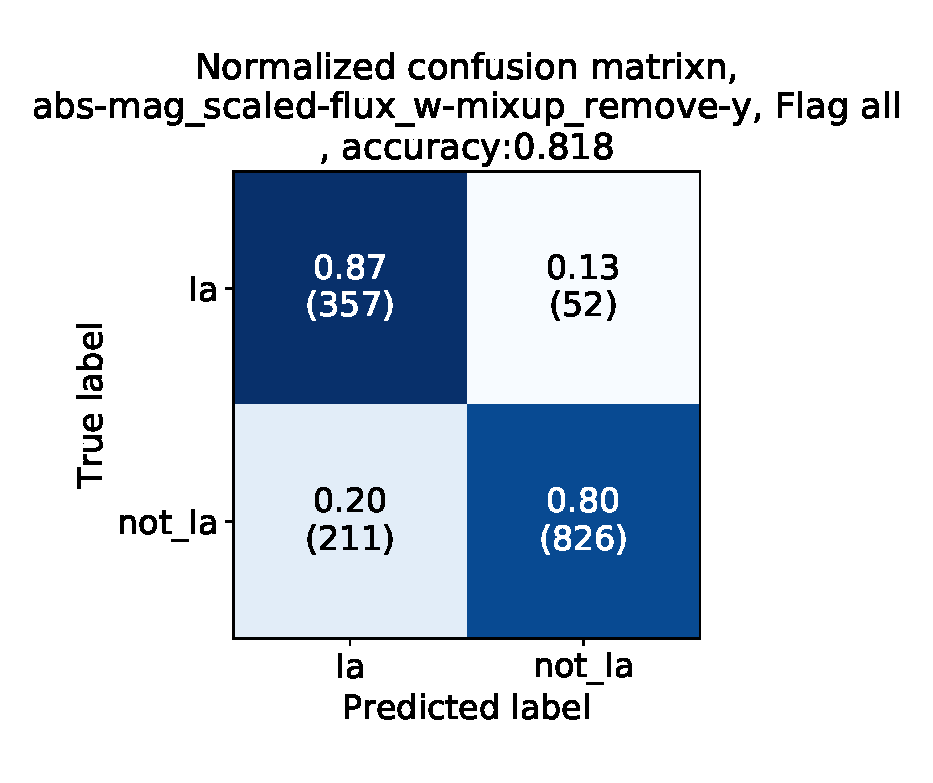
\includegraphics[width=\columnwidth]{figures/10_CM_abs-mag_scaled-flux_w-mixup_remove-y_predictions_test_2_Flagall_all.eps}
            \end{center}
        \end{minipage}
        \begin{minipage}{0.5\hsize}
            \begin{center}
                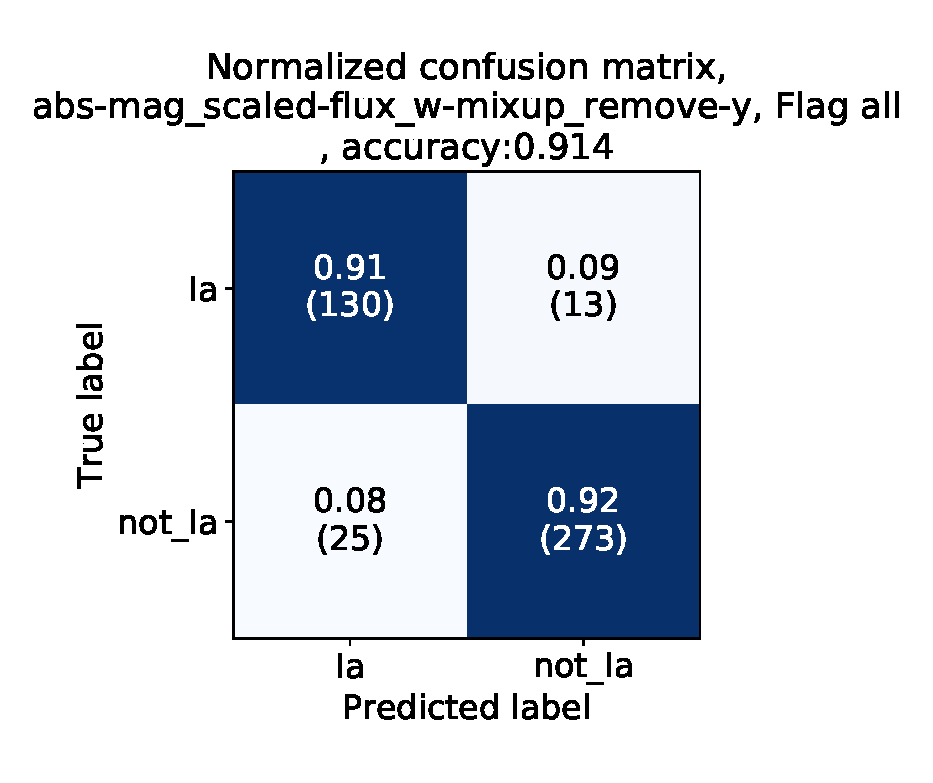
\includegraphics[width=\columnwidth]{figures/10_CM_abs-mag_scaled-flux_w-mixup_remove-y_predictions_test_2_Flagall_noedge_spec.eps}
            \end{center}
        \end{minipage}
    \end{tabular}
    \caption{%
  Confusion matrix in binary classification of All samples (left) and Gold samples (right).
}%
    \label{fig:h2_test_CM}
\end{figure*}
%
%%%%%%%%%%%%%%%%%%%%%%%%%%%%%%%%%%%%%%%%%%%%%%%%%%%%%%%%%
%
\subsection{Multi-type classification}
%
Because we are currently labeling more than three classes for all supernovae detected in HSC transient survey using other methods,
in this paper, we show the classification performance only for the validation dataset with three-class classifier.
%It is necessary to write the reason why there is no answer of multi-class classification.
%
% Classification performance of each model (3class, HSC, validation)
The accuracy for each input in the three-class classification of the validation dataset are summarized in Table\ \ref{tab:h3_validation}.
The best accuracy for the validation dataset is 0.940 in the three-class classification.
The confusion matrix of the best classifier is shown in Fig.\ \ref{fig:h3_validation_CM}.
It represents that our classifier has a very high Sensitivity to Ia supernova while it is not good at classifying Ibc.

In addition, we describe the predicted classes of actual supernovae classified by the three-class classifier.
Figure \ref{fig:h3_class_ratio} shows the predicted class ratio.
Our classifier predicts 1812 supernova classes with a ratio of Ia : Ibc : II = 0.44 : 0.07 : 0.49.
This faraction is between them in volume-limited and magnitude-limited samples in \citet{Li_2011}, which is close to that in volume-limited samples.
However, it should be noted that this ratio is calculated including misclassificaion.
%Table\  summarizes the classification results of all the actual supernova.
%
%Need to write that "ALL" accuracy is weighted
%
%3class Validation
%Ver. 1.2.1
\begin{table}[ht]
\tbl{Accuracy of each input in the HSC three class classification for validation dataset.}{
\begin{tabular}{ccc|p{2em}p{2em}p{2em}p{2em}p{2em}p{2em}}
\hline
\multicolumn{3}{c}{Input} & \multicolumn{6}{|c}{Accuracy} \\
\hline
$M$ & $m$ & $f$  &  Flag\_0 &  Flag\_1 &  Flag\_2 &  Flag\_3 & Flag\_4 &  All \\
\hline
\checkmark &            & \checkmark &        0.985 &        0.926 &        0.920 &        0.890 &        0.774 &         0.940 \\
\checkmark &            &            &        0.971 &        0.894 &        0.886 &        0.844 &        0.729 &         0.914 \\
           & \checkmark & \checkmark &        0.970 &        0.907 &        0.897 &        0.860 &        0.724 &         0.921 \\
           & \checkmark &            &        0.952 &        0.871 &        0.861 &        0.818 &        0.701 &         0.891 \\
\hline
\end{tabular}
}\label{tab:h3_validation}
\begin{tabnote}
* Accuracy for samples extracted from each flag according to the number ratio in the test dataset.
\end{tabnote}
\end{table}
%
%
\begin{figure}[ht]
  \begin{center}
     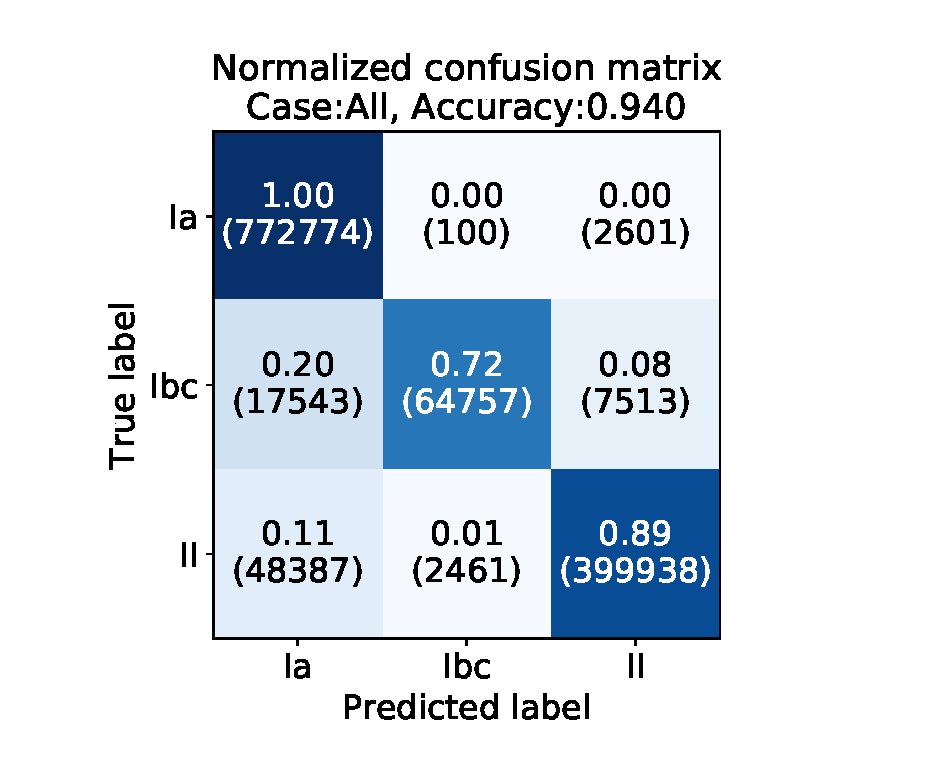
\includegraphics[width=\columnwidth]{figures/13_CM_abs-mag_scaled-flux_w-mixup_remove-y_predictions_validation_2_Flagall_weighted.eps}
  \end{center}
  \caption{%
  Confusion matrix in three-class classification of validation dataset.
  }%
  \label{fig:h3_validation_CM}
\end{figure}
%
%
\begin{figure}[ht]
  \begin{center}
     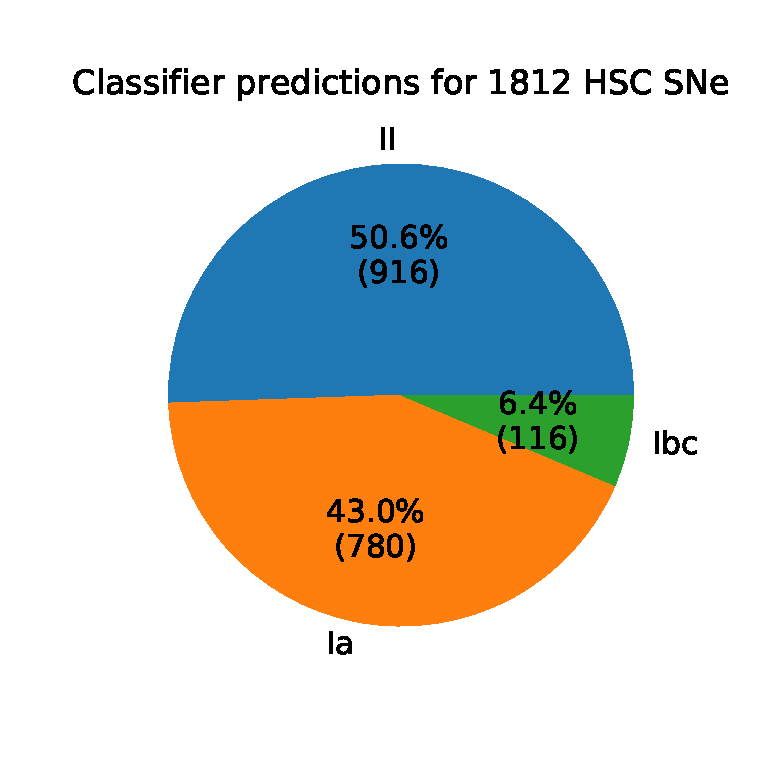
\includegraphics[width=\columnwidth]{figures/14_piechart_hybrid.eps}
  \end{center}
  \caption{%
  Type fractions in the three-class classification of 1812 HSC supernovae.
  }%
  \label{fig:h3_class_ratio}
\end{figure}
%
%%%%%%%%%%%%%%%%%%%%%%%%%%%%%%%%%%%%%%%%%%%%%%%%%%%%
\section{Discussion}
%
\subsection{Comparison with the best classifier in PLAsTiCC}
%
We compare the results of our classifiers and those ranked first place in the PLAsTiCC Kaggle competition.
The best classifier in the PLAsTiCC competition \citep{2019arXiv190704690B} is based on Light-GBM and trained with features extracted from photometric data modeled by Gaussian process regression.
For comparison, we used about 2300 supernova predictions in PLASTiCC data classified by both classifiers.
Since the number of classes to be classified is different between our classifier and the best classifier, we divide the classification results into Ia and the other, and compare as binary classification.
Figure\ \ref{fig:comp_plasticc_1st} shows the confusion matrix of each classifier.
While our classifier and PLATiTiCC 1st classifier cannot be strictly compared because of the different training data sets and number of classification classes,
only for the compared supernovae, our classifier is about 6\% better in total accuracy than the PLAsTiCC 1st classifier and 6\% better in Ia accuracy.
Considering that our classifier only uses the middle one year data out of the original three year data as input, our classifier classifies PLAsTiCC data with better accuracy with less data than that of PLAsTiCC 1st.
However, since our method fixes the observation schedule to input, it is not possible to apply to all PLAsTiCC data with one classifier.
%How many patterns
Our method is not useful for surveys that sweep a wide area like LSST survey, but for surveys that keep observing at the same field of view like HSC transient survey.
%
\begin{figure*}[ht]
    \begin{tabular}{cc}
        \begin{minipage}{0.5\hsize}
            \begin{center}
                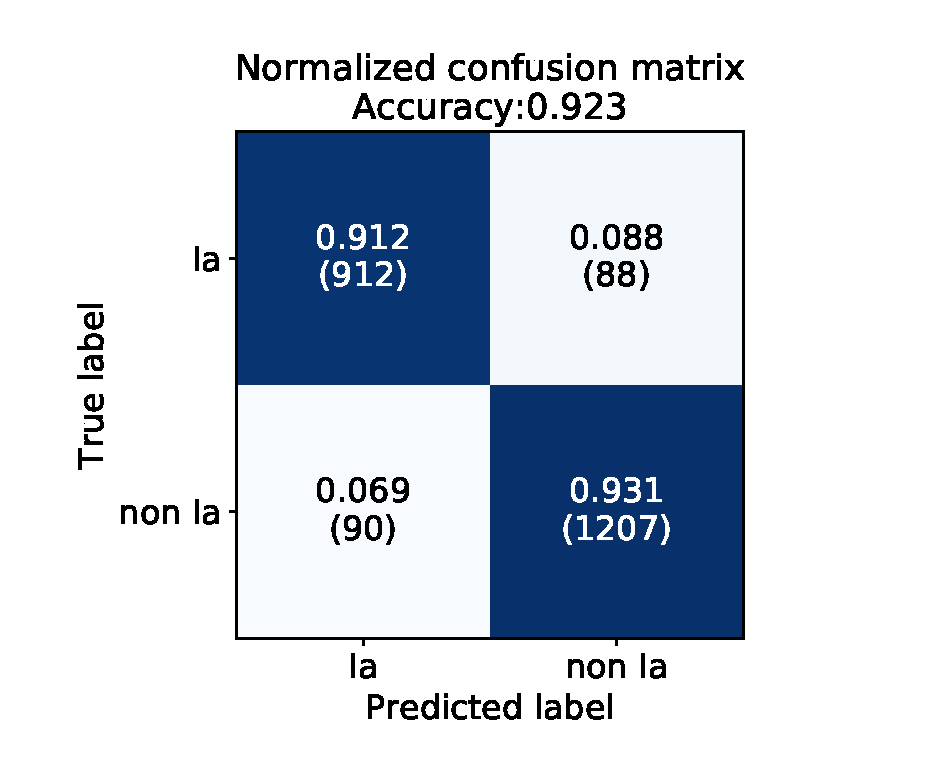
\includegraphics[width=\columnwidth]{figures/07_CM_PLAsTiCC-1st_submission_aug22_2class_2.eps}
            \end{center}
        \end{minipage}
        \begin{minipage}{0.5\hsize}
            \begin{center}
                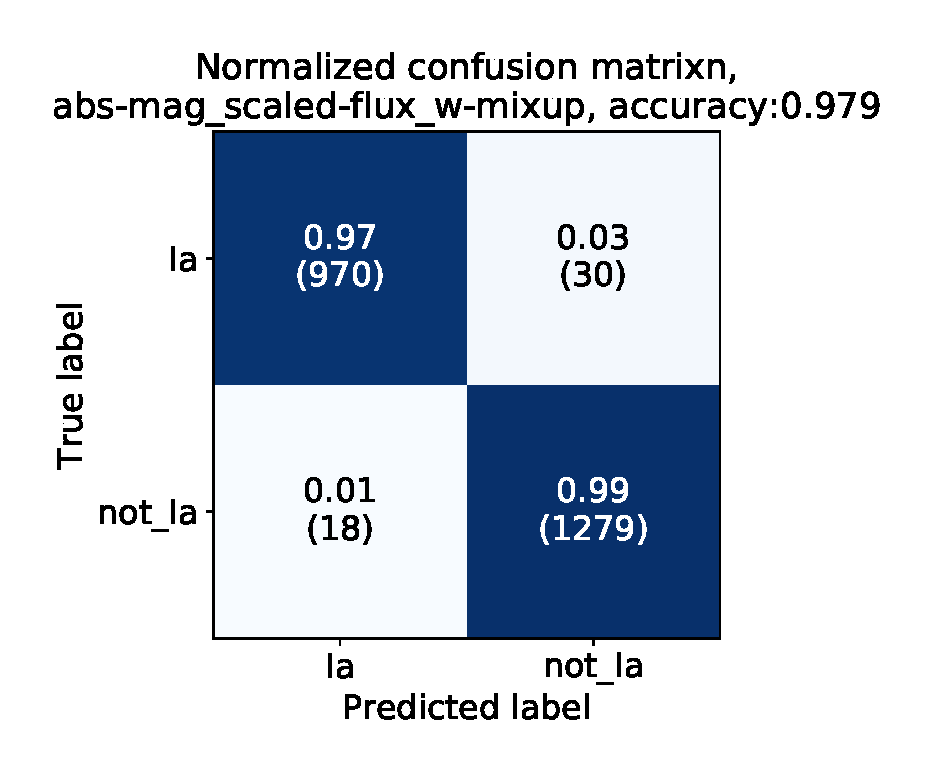
\includegraphics[width=\columnwidth]{figures/03_CM_abs-mag_scaled-flux_w-mixup_predictions_test_2.eps}
            \end{center}
        \end{minipage}
    \end{tabular}  \caption{%
    Confusion matrix in the two-class classification of PLAsTiCC 1st (left) and our classifier (right).
    }%
    \label{fig:comp_plasticc_1st}
\end{figure*}
%
\subsection{Redshift estimation}
%using v1.1.0 results
%
In addition to the supernova type classification,
we also made a redshift estimate using same training dataset for type classification.
The standard deviation of normalized residual $(z_{\rm pred}-z_{\rm spec})/(1+z_{\rm spec})$ \citep{Salvato_2009,Salvato_2019}, used in galaxy photo-z estimation, is applied to the performance criteria for redshift estimation.
In verification with Flag 0 simulated data, that for Ia and non Ia objects are 0.022 and 0.076, respectively.
For the actual HSC supernovae, we used observationally obtained redshifts of host galaxies including spec-z and photo-z for comparison with estimates.
The figure\ \ref{fig:redshift_estimation} shows the comparison between the estimated redshifts and the observed redshifts for the HSC supernovae that the classifier classifies as Ia.
The two classes labeled by SALT2 fit have different distributions, and the events labeled non Ia are less accurate in redshift estimation than Ia.
The normalized residuals for each of Ia and non Ia Flag 0 supernovae labeled with SALT2 fit are normally distributed with standard deviations of 0.066 and 0.138, respectively.
If the comparison is limited to supernovae in the host galaxy with spec-z information, they are 0.056 and 0.130.
Although these estimation accuracy is worse than the template fitting accuracy using host galaxy photometric data, it is useful for selecting host galaxy by comparing the redshift estimated from the supernova light curve itself with those of galaxies.
Furthermore, this distributional difference of residuals leads to the fact that the Ia accuracy can be further improved by excluding events with large residuals in the estimated redshift of the supernova and host galaxy.
%
\begin{figure*}[ht]
    \begin{tabular}{cc}
        \begin{minipage}{0.5\hsize}
            \begin{center}
                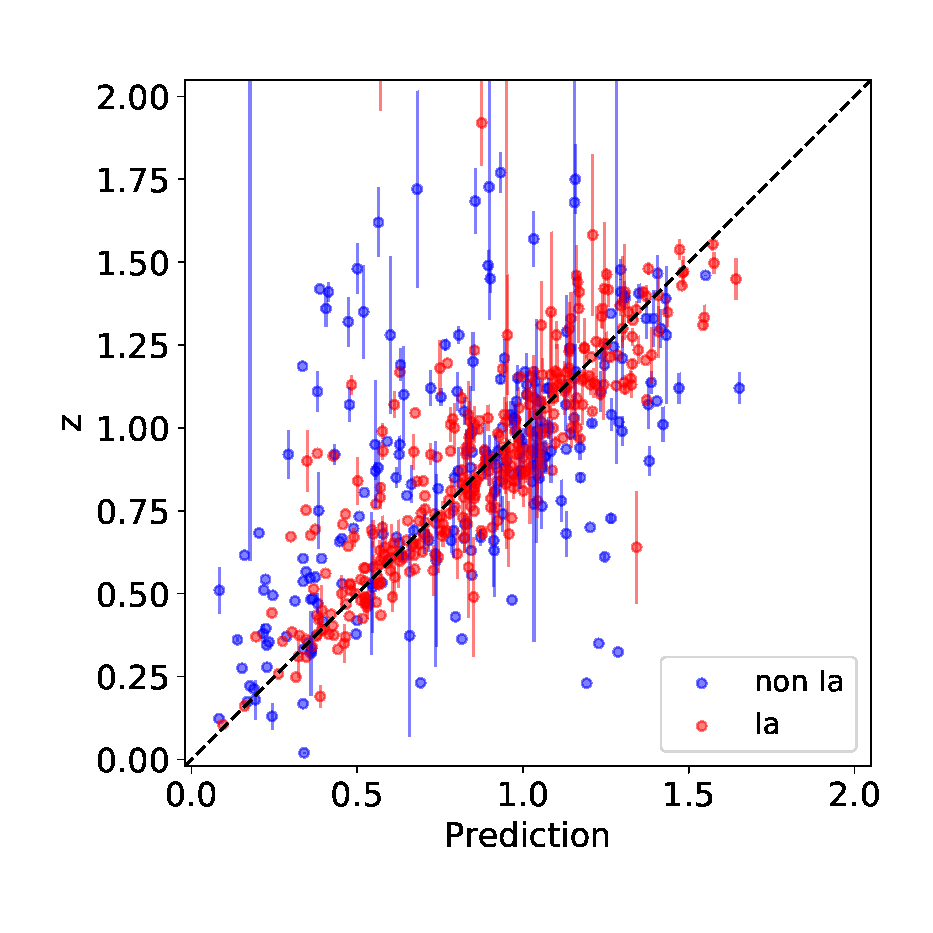
\includegraphics[width=\columnwidth]{figures/redshift_pred_Ia_w_true_label_flagall.eps}
            \end{center}
        \end{minipage}
        \begin{minipage}{0.5\hsize}
            \begin{center}
                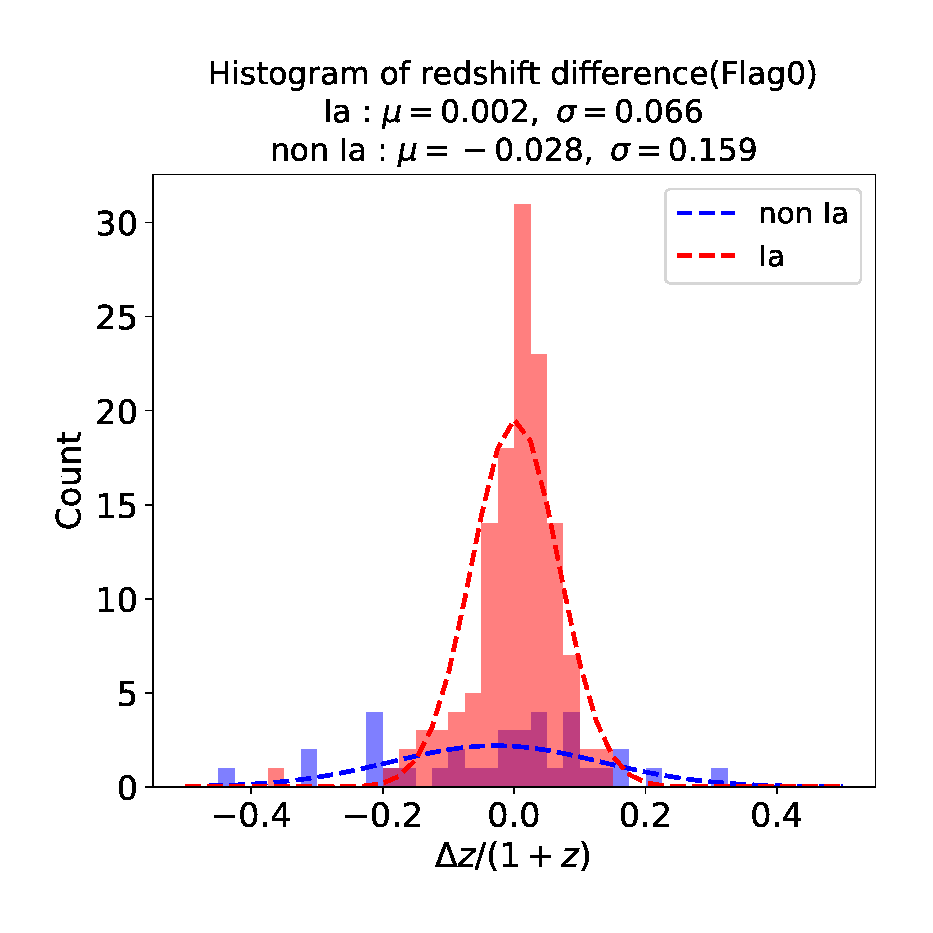
\includegraphics[width=\columnwidth]{figures/redshift_pred_Ia_w_true_label_diff_flag0.eps}
            \end{center}
        \end{minipage}
    \end{tabular}  \caption{%
    (Left) Relation between the machine predictions and the observed redshifts.
    The dashed line is the line of equality.
    The color difference represents SALT-2 fit label.
    (Right) Normalized residual distribution for flag0 supernovae.
    }%
    \label{fig:redshift_estimation}
\end{figure*}
%
%
\subsection{Misclassification}
\label{sec:misclass}
%
Next, we summarize misclassifications in the classification of PLAsTiCC and HSC data respectively.
For PLAsTiCC dataset, misclassified supernovae have the following characteristics:
\begin{itemize}
\item 45\% (46/107) of them do not include the supernova peak phase in the photometric data, while they are only 22\% of all events.
\item Many others have similar probabilities.
\item Most of quite wrong events misclassify Ibc as Ia or II.
\end{itemize}
The figure\ \ref{fig:misclass_rate_3class} shows the misclassification rate against redshift for the PLAsTiCC dataset.
In the three-class classification of the PLAsTiCC data set, we found that the accuracy of Ibc was lower than that of other classes, and that the accuracy dropped significantly in the vicinity of redshift 1.0, and in addition, the accuracy also decreased for nearby Ibc supernovae.
While some misclassified supernovae are so dark and indeterminate that they are difficult to classify even with traditional methods,There are also bright supernovae that are completely misclassified.
In the binary classification of the HSC gold samples, 13 Ia labeled supernovae are classified as non Ia.
Four of them are boundary events which have Ia probability of 40 to 50\%.
Five of the remaining nine are events with relatively few input data points belonging to Flag1 and Flag3.
The other supernovae have outlier values and poor photometry components.
%
\begin{figure}[ht]
  \begin{center}
     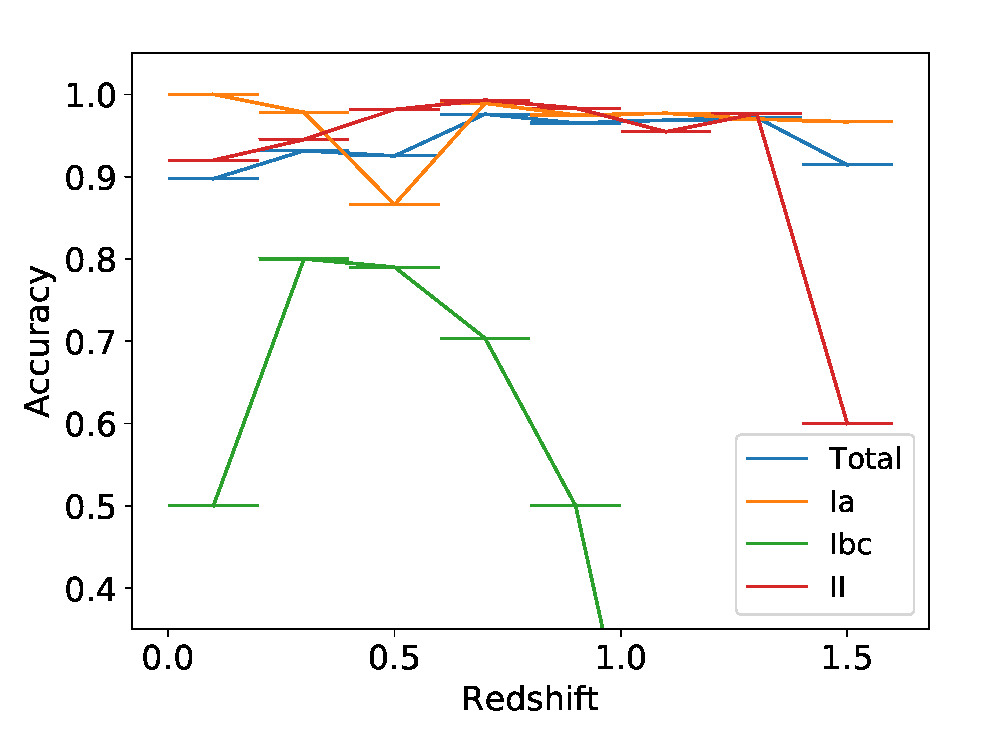
\includegraphics[width=\columnwidth]{figures/misclass_rate_plastic_3class.eps}
  \end{center}
  \caption{%
  Misclassification rate against redshift
  }%
  \label{fig:misclass_rate_3class}
\end{figure}
%
%
\subsection{Performance depending on input configuration}
%
When using our classification method, the number of dimension input to the classifier, the number of photometric data points, increases as the survey progresses in the actual survey.
Therefore, we discuss about the transition of performance against the number of inputs.
We classified the HSC dataset by increasing the number of input dimensions one by one, and investigated the relationship between the number of input photometric data pionts and the classification performance.
Binary classifiers are used for classification, and evaluation is performed using accuracy calculated from the confusion matrix.
The figure\ \ref{fig:n_observations} shows the transition of classification performance along with the number of inputs.
Although the Ia accuracy is as low as 0.6 to 0.7 in the early stage of the survey with less than five inputs, it exceeds 0.8 when the number of inputs increases to 20.
The partial decrease in accuracy is thought to be due to the new supernova found at the added photometric point.

By regrouping all events classified while changing the number of input dimensions into groups according to the length of the supernova detection period, we investigated the classification performance for each phase from the rise of the supernova.
The figure\ \ref{fig:n_observations_SNphase} shows the classification performance against the supernova phase.
This figure presents how long supernova photometric data is needed to classify with high accuracy using our classifier.
As mentioned in section \ref{sec:misclass}, the classification performance is low if only the initial rising phase before the supernova peek is included in the input photometric data, but the accuracy increases to 90\% when we input two weeks of supernova data from the first detection.
Since the observation interval in the HSC survey is not constant, the number of inputs may be different even for supernovae with the same detected period.
Due to this fact, there is a variation in the average input dimension number of samples in each phase, which causes a fluctuation in accuracy.
In addition, from the cumulative number of supernovae classified as Ia with high probability,  it is estimated that our classifier can classify two or three Ia supernovae candidate to follow-up in one month observation.'

Lastly, we discuss the transition of the Ia probability output by the classifier along the supernova phase.
Each time the supernova photometric data input to the classifier increases, Ia probability, the output of the classifier, is updated.
For each of 100 supernovae labeled Ia and non-Ia with SALT2 fitting, we extracted its Ia probability for each duration from the various classification results, and plotted its transition as Figure\ \ref{fig:n_observations_SNphase}.
Although the Ia probability fluctuates greatly in the earliest phase, it begins to divide in about two weeks, and it can be clearly separated in one month.

%
\begin{figure}[ht]
  \begin{center}
     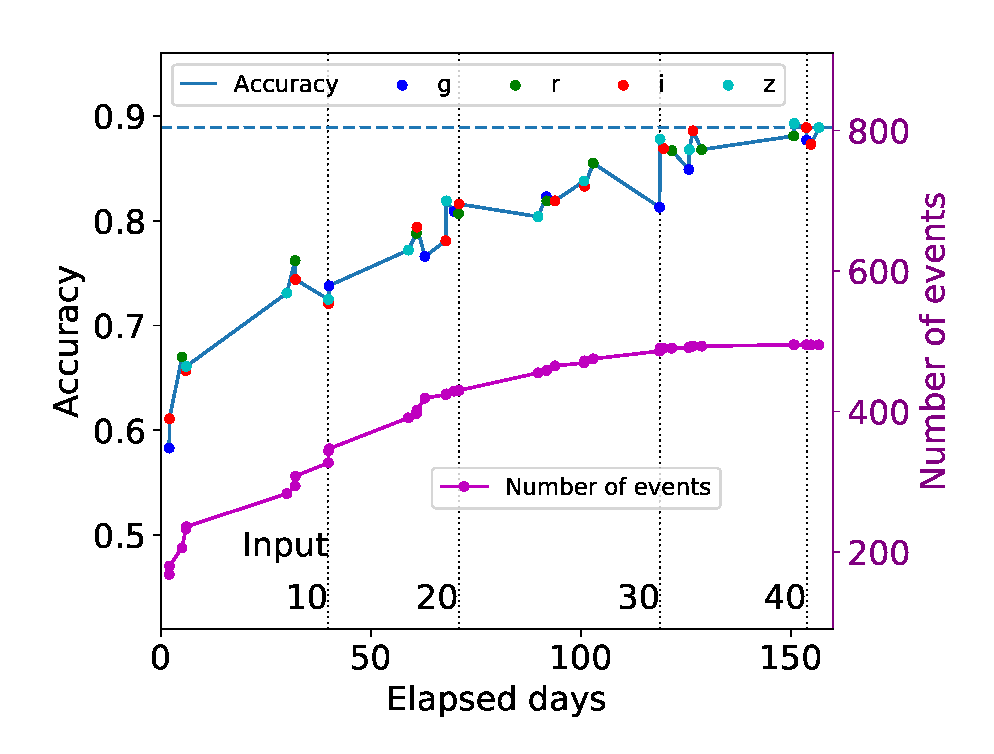
\includegraphics[width=\columnwidth]{figures/n_observations_v2.eps}
  \end{center}
  \caption{%
  Relationship between the number of inputs to the classifier and classification performance in binary classification for HSC datasets. 
  The horizontal axis is the elapsed days of HSC survey, and the vertical dot line shows the scale of input photometric point number. 
  The color of each mark in accuracy indicates the band of the added photometric point.
  }%
  \label{fig:n_observations}
\end{figure}
%
%
\begin{figure}[ht]
  \begin{center}
     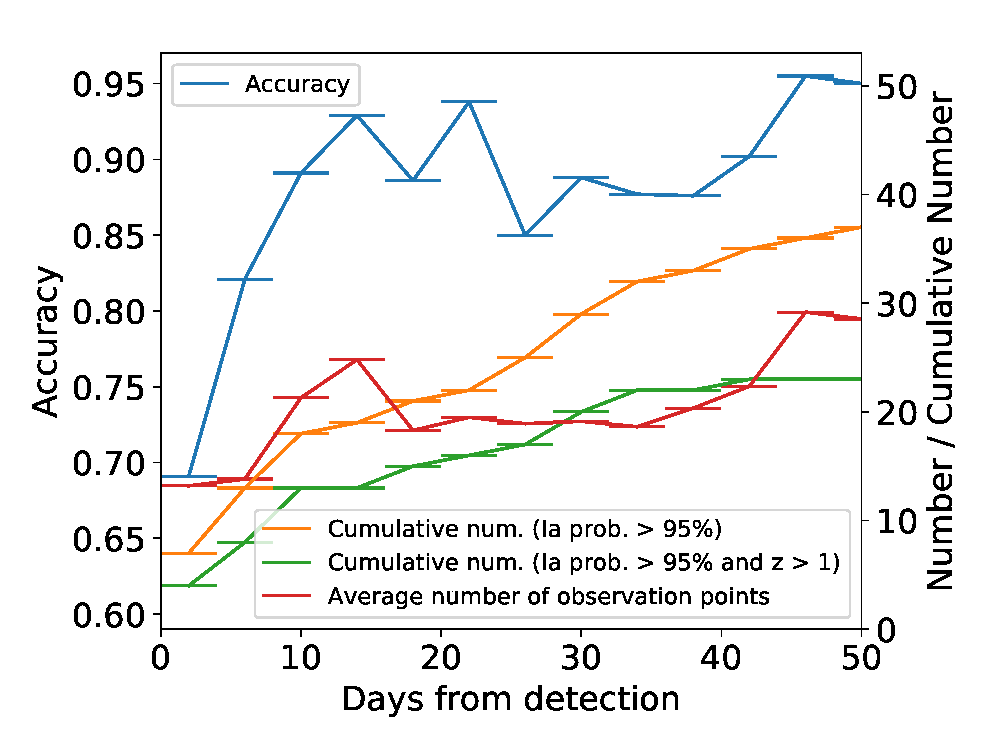
\includegraphics[width=\columnwidth]{figures/n_observations_SNphase_191114.eps}
  \end{center}
  \caption{%
  Classification accuracy and cumulative number of type Ia supernovae classified with high probability against supernova phase.
  The orange line indicates the number of supernovae with Ia probability $>$ 95\%, and green line are that for distant supernovae at z $>$ 1. Average number of observation points with red lines.
  }%
  \label{fig:n_observations_SNphase}
\end{figure}
%
%
\begin{figure}[ht]
  \begin{center}
     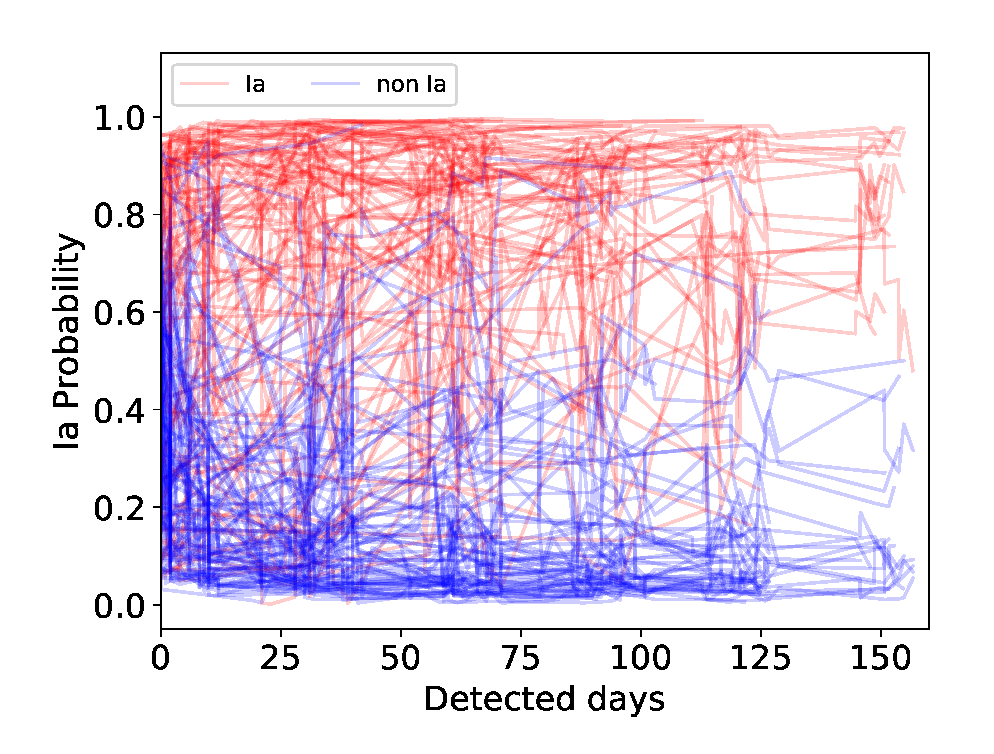
\includegraphics[width=\columnwidth]{figures/n_observations_visualized_Ia_probability_line.eps}
  \end{center}
  \caption{%
  Transition of Ia probability with increasing elapsed time of input supernovae
  }%
  \label{fig:visualized_Ia_prob}
\end{figure}
%
%
\section{Conclusion}
%\begin{itemize}
%\item 
%\item 
%\item our new method(2DGP+LGBM)
%\end{itemize}
%
In this paper, we present a model of a classifier that classifies supernova types by directly inputting photmetric data and its classification performance.
Our DNN classifier trains with simulated supernova photometric data from PLASTiCC templates and classifies PLASTiCC data and HSC survey actual supernova data with high accuracy of 0.95 and 0.90 respectively.
The discussion on the number of input dimensions also shows that our classifier can classify the HSC survey data with sufficient accuracy even with only pre-peak data about two weeks after the first detection.
From these facts, we conclude that this classifier has sufficient classification performance for subsequent type-specific studies and selection of follow-up targets even in actual HSC surveys.
Our method is specialized in the HSC survey in which each observed transient tends to have the same cadence by observing a certain region deeply.
It can use all photometric information and classify almost without any pre-processing, compared to the method of reducing dimensions and extracting features. However, this method is not good at dealing with differences in observation schedules for each classification object.
To classify all objects with our method, we need to prepare multiple classifiers.
In order to support ultra-wide-range surveys such as LSST, it is necessary to input features that are less affected by the magnitude of the cadence for each transient, and to add processing to interpolate missing values.
However, our proposed method is easy to apply to estimation models such as redshift because of simple input. The application of our model to redshift estimation is useful for the selection of host galaxies by comparing with the photo-z information of galaxies.
What we found out by classifying actual data with our method is that there is a difference in the results of validation and test set.
Of course, the labeling of the actual data class by the conventional method includes uncertainty, but the difference in the results should be minimized by making the learning data more similar to the actual data.
%
\begin{ack}
 a brief note for an acknowledgment, if any.   
\end{ack}
%
\bibliographystyle{myaasjournal}
\bibliography{hsc,archive}
%
\end{document}
